\documentclass[11pt, a4paper]{memoir}
\usepackage[utf8]{inputenc}
\usepackage[english, science, dropcaps, hyperref, submissionstatement]{ku-frontpage}

% Math-related packages
\usepackage{amsmath, amssymb, amsfonts, mathrsfs, latexsym, mathtools}
\usepackage{ntheorem}
\usepackage{tikz}
\usepackage[framemethod=TikZ]{mdframed}
\usepackage{centernot}
\usepackage{tikz-cd}
\usetikzlibrary{arrows.meta, decorations.pathreplacing, bending,patterns}


% Miscellaneous packages
\usepackage{enumitem}
\usepackage{float}
\usepackage{xcolor}
\usepackage{etoolbox}
\usepackage[most]{tcolorbox}
\tcbuselibrary{theorems, skins, breakable}
\usepackage{ulem}
\usepackage{microtype}
\usepackage{setspace}
\usepackage{graphicx, caption}
\usepackage{chngcntr}
\usepackage{cleveref}
\definecolor{emphcolor}{HTML}{901A1E} % Using kuRed

\newcommand{\coloremph}[1]{\textcolor{emphcolor}{\emph{#1}}}

\DeclareCaptionStyle{mystyle}{%
  font=it, % Italif font
  labelsep=space, % Use space instead of colon
  justification=RaggedRight % Left-align the caption
}
\captionsetup{style=mystyle}
\captionsetup{belowskip=-15pt}

\crefformat{footnote}{#2\footnotemark[#1]#3}
\counterwithout{figure}{chapter}

% Theorem-like environments with italicized text
\theoremstyle{break}
\theoremheaderfont{\normalfont\bfseries}
\theorembodyfont{\itshape} % Italicized text
\theoremseparator{.}

\newtheorem{thm}{Theorem}
\newtheorem{prop}{Proposition}
\newtheorem{cor}{Corollary}
\newtheorem{lem}{Lemma}

% Definition environment with non-italicized text
% Definition environment with non-italicized text
\theoremstyle{break}
\theoremheaderfont{\normalfont\bfseries\vspace{3pt}}
\theorembodyfont{\normalfont} % Non-italicized text
\theoremseparator{.}
\newtheorem{innerdefn}{Definition}

\newenvironment{defn}
  {\begin{innerdefn}}
  {\ensuremath{\circ}\end{innerdefn}}
  

\newtheorem{inneralg}{Algorithm}
\newenvironment{alg}{\begin{inneralg}}{\ensuremath{\circ}\end{inneralg}}  

% Alternative definition environment
\definecolor{kuRed}{HTML}{901A1E}
\definecolor{kuGray}{HTML}{666666}
\definecolor{lightKuGray}{HTML}{FFE8D1}

% Define the 'mydefinition' tcolorbox environment
\newtcolorbox[auto counter,number within=chapter]{mydefinition}[2][]{
  breakable, % Allows the box to break across pages
  colback=lightKuGray!80, % Background color for the entire box
  colframe=lightKuGray!80, % Frame color
  coltitle=black, % Text color for the title
  title={\textbf{Definition~\thetcbcounter\ (#2)\ #1}}, % Title with bold "Definition" and optional description
  fonttitle=\bfseries, % Make the title text bold
  enhanced,
  sharp corners,
  boxrule=1pt, % Width of the frame lines
  top=8pt, % Top space within the box (inside the frame)
  bottom=8pt, % Bottom space within the box (inside the frame)
  left=8pt, % Left space within the box (inside the frame)
  right=8pt, % Right space within the box (inside the frame)
  toprule=10pt,
  before=\vskip15pt,
  after=\vskip15pt,
  #1 % For specifying additional options
}

\theoremstyle{nonumberplain}
\theoremsymbol{\ensuremath{\square}} 
\newtheorem{proof}{Proof}

% Custom commands and math operators
\newcommand{\mN}{\mathbb{N}}
\newcommand{\mZ}{\mathbb{Z}}
\newcommand{\mQ}{\mathbb{Q}}
\newcommand{\mR}{\mathbb{R}}
\newcommand{\mD}{\mathbb{D}}
\newcommand{\mH}{\mathbb{H}}
\newcommand{\mC}{\mathbb{C}}
\newcommand{\mP}{\mathbb{P}}
\newcommand{\mF}{\mathbb{F}}
\newcommand{\abs}[1]{\left| #1\right|}
\newcommand{\norm}[1]{\left\lVert#1\right\rVert}
\newcommand{\indep}{\perp \!\!\! \perp}

\DeclareMathOperator{\pa}{pa}
\DeclareMathOperator{\de}{de}
\DeclareMathOperator{\nei}{ne}
\DeclareMathOperator{\bd}{bd}
\DeclareMathOperator{\nd}{nd}
\DeclareMathOperator{\an}{An}
\DeclareMathOperator{\supp}{supp}
\DeclareMathOperator{\rank}{rank}
\DeclareRobustCommand{\firstsecond}[2]{#2}

% Other settings
\setlength\arraycolsep{2 pt}
\setcounter{tocdepth}{2}
\setcounter{secnumdepth}{1}
\setlength{\jot}{8pt}

\assignment{Master's thesis}

% The following are only needed if the \author, \title, \subtitle, and \date
% commands are not patchable. See the readme for more information.
% \frontpageauthor{Alex Author}
% \frontpagetitle{A concise but nevertheless\\precise and interesting title}
% \frontpagesubtitle{An intruiging subtitle}
% \frontpagedate{Submitted: \today}

\frontpagetitle{Causal Inference in Dynamic Systems}
\subtitle{Convergent Cross Mapping and Alternative Approaches}
\frontpageauthor{Rasmus Juhl Christensen}
\frontpagedate{Submitted: \today}
\advisor{Advisor: Niels Richard Hansen}
\frontpageimage{example.png}

\kupdfsetup{A concise but nevertheless precise and interesting title - An intruiging subtitle}{}{Alex Author}

\begin{document}
\begingroup
  \fontencoding{T1}\fontfamily{LinuxLibertineT-OsF}\selectfont
  \maketitle
\endgroup

\section*{Abstract}
\addcontentsline{toc}{section}{Abstract}


\subsubsection*{Description from contract}
The main goal of the project is to investigate dynamic systems for time series and the effectiveness of convergent cross mapping (CCM) to detect causality in this framework compared to other approaches on the basis of a reference model. Drawing on the paper "Detecting Causality in Complex Ecosystems" (2012) and "Distinguishing time-delayed causal interactions using convergent cross mapping", the project will explore the theoretical foundations, practical applications and potential shortfalls of CCM and its link to more classical methods in causality.\\\\
Reference 1: Detecting Causality in Complex Ecosystems. George Sugihara, Robert May, Hao Ye, Chih-hao Hsieh, Ethan Deyle, Michael Fogarty and Stephan Munch. Science , 26 October 2012, New Series, Vol. 338, No. 6106 (26 October 2012), pp. 496-500.
Reference 2: Distinguishing time-delayed causal interactions using convergent cross mapping. Hao Ye, Ethan R. Deyle, Luis J. Gilarranz \& George Sugihara. Scientific Reports volume 5, Article number 14750, 2015.\\\\
 
\textit{Front page image generated by Chaoscope.}
\newpage
\tableofcontents


\vfill
\noindent All code and data used in this project is available at \url{github.com/juhlc/speciale}.

\normalem

\newpage

\chapter{Introduction}
Causality is a cornerstone of understanding in various scientific domains, and at its core, causal inference addresses the intricate dance between correlation and causation. While correlation hints at a mutual relationship between two variables, causation pushes us into the territory of assertion — \textit{does one variable truly influence the other?} Traditional statistics employs randomization as a useful tool. Imagine a medical scenario where you can control who receives a treatment: If you can ensure that it is perfectly random who receives the treatment and patients receiving the treatment consistently show improvement compared to those who don't, we can easily attribute that difference to the treatment. However, when variables are merely observed without that level of control, establishing causation becomes more complex. Causal statistics thus requires another level of statistical modelling, because we want to reason about what happens when intervening in the process.\\\\
This thesis delves into the vibrant world of causal relationships in dynamic systems. Granger causality, a seminal and widely used concept in causal analysis of time series, yields one approach to causal inference in time-dependent data. It is based on the thoughts of \cite{Granger}, and it posits that if the past of a variable $C$ contains unique information about another variable $E$, the variable $C$ is said to 'Granger-cause' the variable $E$. This approach to causal inference is based on prediction and at its core, it operates on the principle that cause precedes effect, which means that knowledge of the cause can enhance the predictability of the effect. However, while Granger causality offers a framework for assessing causality in probabilistic settings, it encounters challenges in deterministic systems. Dynamic systems, by nature, have variables that are interconnected and governed by underlying structures. This interconnectedness means that information about one variable can often be extracted from another due to the system's inherent dynamics, rather than any direct causal link.\\\\
A case in point is the result from \cite{Takens} which suggests that observing a single variable from a dynamic system might be sufficient to capture the entire system's dynamics. This interconnectedness can lead Granger causality to mistakenly identify causal links where none exist. Enter now the deterministic systems' viewpoint: Instead of relying on simple prediction improvement as a marker of causality, we focus on the inherent information within variables. If variable 
$C$ causes variable $E$, then $E$ should encapsulate information about the dynamics of $C$. However, $C$ would not necessarily contain comprehensive information about $E$, as it would not include information about the dynamics of $E$ not imposed by $C$. This perspective flips Granger causality on its head: while Granger causality might predict the effect 
$C$ using the cause $E$, a deterministic viewpoint effectively suggests the opposite. \\\\
This distinction, subtle, yet profound, reshapes our understanding of causality in dynamic systems. As we proceed, we will delve deeper into the theoretical underpinnings of this perspective, unpacking its implications and potential applications. In particular, this insight leads to the \emph{Convergent Cross Mapping} approach introduced by \cite{Sugihara}, which serves as both the motivational starting point and the culmination of the theoretical work based on Takens' theorem in this thesis. A detailed discussion of this approach is presented in Chapter \ref{chapTaken}.\\\\
Yet, while the deterministic paradigm offers a fascinating lens through which to understand causality, there is an inherent limitation. Real-world systems, especially in fields like economics, biology, and climate science, are rife with unpredictable fluctuations. These fluctuations cannot always be attributed solely to the endogenous dynamics of the system. No matter how meticulously one captures the deterministic dynamics, there will always be elements of seeming randomness and external influences that a purely deterministic model would struggle to account for. We return thus to stochastic processes. By reintroducing a stochastic element into our models, we can more faithfully represent the unpredictability and variability inherent in real-world systems. Stochasticity provides a framework to account for the 'noise' that isn't explained by the deterministic components of a system. Moreover, it's a nod to the humility of our modelling efforts – recognizing that there are always aspects of complex systems that are beyond our current understanding or inherently random. 
In the subsequent chapters, we will delve deeper into the fusion of deterministic dynamics with stochastic processes using  a mixture of simulation based methods and theoretical considerations seeking a harmonious balance that brings us closer to understanding the multifaceted nature of causality in dynamic systems.
\newpage
\section{An Example}
To illustrate the challenge of causal inference in complex dynamic systems, we will use a real-world example concerning interactions between anchovies, sardines and sea surface temperature in the California Current ecosystem. This example serves as a backdrop for the more theoretical nature of the rest of this thesis. In keeping with the analysis of \cite{Sugihara}, we aim to use the same data for our analysis but we do extend it by including data from the period 2012-2022 as well. The data consist of the following variables:
\begin{itemize}
\item Pacific sardine (\textit{Sardinops sagax}) California fish market catch landings recorded monthly in pounds in the period January 1928 up to and including December 2022. There are 12 months with redacted data.\footnote{\label{note1}Data from January 1928 up to and including December 2002 is obtained from from \textit{ERDDAP} at \cite{oldData}, and data from January 2003 up to and including December 2022 is obtained directly from \cite{newData}.}
\item Northern anchovy (\textit{Engraulis mordax}) California fish market catch landings recorded monthly in pounds in the period January 1928 up to and including December 2022. There are 34 months with redacted data.\cref{note1} 
\item  Sea-surface temperature (SST) measured daily in $\text{C}^\circ$ as an average between temperatures measured at the two sites Scripps Pier Shore Station and Balboa Pier Shore Station in the period August 22, 1916 up to and including December 31, 2022. There are 458 days without any measurements at either site.\footnote{The data from Scripps Pier is maintained by \cite{Scripps} and covers the period from August 22, 1916 up to and including December 31, 2022. The data from Newport Pier is maintained by \cite{Newport} and covers the period November 1, 1924 up to and including December 31, 2022.} 
\end{itemize}
Commercial landings data is considered confidential and therefore some landings recordings have been redacted due to insufficient data to summarize and maintain confidentiality.\footnote{This is a consequence of the California Fish and Game Code Section 8022. See: \url{https://wildlife.ca.gov/Conservation/Marine/Data-Management-Research/MFDE/User-Guide}} We will set landings in all months with redacted data to zero considering the reason for redaction. As for the temperature data, we impute missing data with surrounding data points on the reasoning that temperature probably does not vary significantly from day to day and that any specific day does not carry significant weight in yearly averages. Since the particular question in hand is not of significant interest for the thesis itself and only intended to be an illustration of the systems we intend to study, we shall not consider any implications of these choices in this thesis. For a comprehensive study of the interdynamics of sardine and anchovy populations, we refer to \cite{Sardine}.\\\\
We will use the landings data as a proxy for the population size of sardines and anchovies. This, of course, does entail some problems, since we have no measurements of the populations themselves and will result in some uncertainty, but we will disregard this discussion since it is not of inherent interest to the topic. To visualize the data, we plot the annual landings of sardine and anchovy alongside trend lines computed as the 3-year averages and the 3-year averages of the SST:
\begin{center}
	\begin{figure}[!ht]
		\includegraphics[width=\textwidth]{{"../r code/sardine"}.png}
		\caption{}
	\end{figure}
\end{center}
We observe a noticeable collapse in the sardine population in the 1960's coinciding with a rapid growth of the anchovy population. In fact, there seems to be a significant negative correlation between sardine and anchovy landings in most of the 20th century. This phenomenon was not exclusive to the Califonia Current System, where the sardine ecosystem experienced an almost total ecological collapse as described in \cite{Sardine}. It was hypothesized in the 1970's that internal competition between the two species was a driving factor in the dynamics of the system,  see for instance \cite{Compete}. In some places, the theory of interspecies competition led to suggested policies of subjecting the anchovy to heavy fishing pressure hoping that this would benefit the sardine ecosystem. Approaching the 21st century the presumed negative correlation between sardine and anchovy populations seemed to disappear and and even change sign thus illustrating a feature of dynamic systems: variables can appear to be correlated, but over time this correlation may vanish or change sign. This phenomenon is named \textit{mirage correlation} by \cite{Sugihara}. This also serves as a reminder of the well-known fact that correlation does not imply causation. Moreover, we observe that the SST has  risen sharply in recent years consistent with global warning which is something that could impact findings based on this data.\\\\
To further illustrate the relationship between SST and the landings data, we transform the landings data to log-returns, i.e. the time series $(X_t)_{t\in T}\in \mR_+^T$ is transformed as follows
$$(X_t)_{t\in T} \mapsto \left(\log\left(1+\frac{X_t-X_{t-1}}{X_{t-1}}\right)\right)_{t\in T}\approx \left(\frac{X_t-X_{t-1}}{X_{t-1}}\right)_{t\in T}$$
The approximation on the right is valid when $(X_t-X_{t-1})X_{t-1}^{-1}$ is small, and thus the log-returns indicate the relative difference from year to year while shrinking very large positive values, which appear often in our data set. Below we plot the log-returns alongside 3-year averages and a scale of the 10-year average SST computed in each year as the average of the 10 previous 10 years:
\begin{center}
	\begin{figure}[!ht]
		\includegraphics[width=\textwidth]{{"../r code/diff"}.png}
		\caption{}
	\end{figure}
\end{center}
The apparent patterns in the previous figure are significantly less obvious now. A negative correlation between sardine and anchovy populations is indeed less pronounced now, although we do see some spikes in opposite directions around 1970 and 1980. More pronounced is the lower level of the averages of the SST in the 1960's, and the return of the sardine population coinciding with the decline of the anchovy population and the return of higher average SST's. The climate and ecological changes connected with the development in sea surface temperatures are also deemed to be driving the population changes in the analysis done by \cite{Sardine}. We observe that a potential causal relationship between temperature and sardine and anchovy landings is \textit{regime dependent} or \textit{state dependent} thus revealing another feature of dynamic systems. In the recent warmer years, the previous dynamic between temperature and population sizes seems to disappear. This resembles the phenomenon of mirage correlation. In fact, the State of California introduced legislation in the 1990's aimed at protecting the sardine population, which implemented restrictions based on temperature. This was suspended in 2010 due to rising sea surface temperatures.\\\\
We see that the log-returns look fairly stationary over time and one approach could be to analyze this data with standard techniques based on Granger causality in time series data. Let $X_t\in \mR^3$ denote the values of the log-return of sardine, the log-return of anchovy and the average of sea surface temperature at time point $t$. We then introduce the VAR($p$)-model for this system:
$$X_t=A_1 X_{t-1}+A_2 X_{t-2}+\cdots + A_p X_{t-p}+u_t$$
where $A_1,\ldots, A_p\in \mR^{3\times 3}$ are coefficient matrices and $u_t$ is a noise term. The coefficient matrices can be estimated with OLS (which is also the maximum likelihood estimator when assuming that $u_t$ is normally distributed and mean-zero), and we can get standard confidence intervals based on an assumption of asymptotic normality. We see that the matrices model the influence of past values of all variables on the present values of the variable in question. For now, we will cautiously endow this influence with a causal interpretation, although the nuances of this interpretation is yet to be made explicit. At the very least, we will take it as an indication of a possible causal link.\\\\ 
We have to choose the parameter $p$ specifying the number of lags in the model. This can be done by choosing the model according to a minimal information criterion like AIC. Fitting a VAR(1) model with first-differenced temperature data to the data, yields an estimate of $-2.6$ of the coefficient from temperature to anchovies and an estimate of $17.9$ of the coefficient from temperature to sardines. The remaining coefficients for sardine and anchovy are all estimated to $0.0$. No coefficient is significant 95\% level, but this is expected due to the small sample size. However, this does indicate that temperature might positively influence the sardine population and negatively influence the anchovy population. We are looking at averages of temperature over a 10-year period; any window of averaging in the range from 5 to 10 years does not change the sign and size of the estimates significantly, but when looking at the yearly averages of temperature alone, we no longer get estimates that does not round to 0. This shows that the indication is not just a happy accident, although we lack power to say anything definitively.\\\\ 
These results do not, however, exploit some of the properties of dynamic systems that we observed and discussed above, and the present approach does require some data manipulation in order to use standard econometric methods. Notice for instance, that a VAR($p$)-model under standard assumptions entail a stationary time series which means that we have to look for transformations of our time-series yielding this property or at least something that can reasonably me modelled with a stationary time series. Here, this is achieved by the standard transformation, but it is a model assumption that needs addressing. This is the inspiration for the work that we will now undertake.


\chapter{Causal Models}
In this chapter, we will introduce approaches to causal modelling and compare corresponding definitions of causation. In the process we will try to illuminate the underlying motivations. We rely on the fundamental understanding of causality as the characterization of the effect of interventions in a system of variables, and we shall build our models on the back of graphical models. We will also introduce the causal framework of structural causal models inspired by the account of \cite{Peters}. This framework not only offers a model for causal inference but also a guideline for formulating a causal language for models in a deterministic setting. Due to the inherent differences between the mathematical theory used to formulate models in stochastic and deterministic settings, we will aim to relate the underlying assumptions in each setting. However, we will inevitably encounter some conceptual problems, as any attempt to translate the philosophical concept of causality into mathematical terms will be endowed with non-trivial complications and notable exceptions. We will discuss these problems throughout as they arise and try to be explicit about the assumptions and potential problems of the causal framework chosen in this thesis. We will also briefly discuss alternative formulations less conducive to overly strong interpretations. In doing this, we follow the conventions of causal graphical  models as pioneered by \cite{Spirtes} and \cite{Pearl}, and, of course, inspired by the work of \cite{Steffen}.
\section{A Simple Causal Model}
In that vein, one such approach to formalization is that of the \textit{Structural Causal Model (SCM)}, inspired by the terminology \cite{Peters}, which in its most simple form can be formulated for two variables as
\begin{align*}
C&\coloneqq N_C\\
E&\coloneqq f(C,N_E)
\end{align*}
where $N_C,N_E$ are independent random variables of some distribution and $f$ a suitable function. In this case, we denote $C$ the cause and $E$ the effect. We shall think of these expressions as assignments and not merely equations fulfilled by the variables of the system. By this, we mean that we think of $E$ being \textit{generated} as the functional expression of $C$ and a noise term and not that it fulfils this property by accident, from some equilibrium condition or other such imaginable circumstances. For now, this is not mathematically relevant, but it does guide how we should think of interventions. If we believe these equations to be the result of some equilibrium, then we would not necessarily expect an intervention in $C$, such as fixing its value to $C\coloneqq c$, to produce the effect that $E$ is now given by $E\coloneqq f(c,N_E)$. On the other hand, if we interpret these expressions as assignments, this should be the expectation under the model. This marks a difference to the seemingly identical \textit{Structural Equation Model (SEM)} that is favoured in the field of econometrics. In the setting of SEMs, it is less obvious how to think of interventions, but we will return to the intricacies of this distinction later on. In either case, we notice that the expressions above entail a joint distribution of $C$ and $E$. An obvious deficiency is that the representation above is not unique in the sense that varying the function and noise terms can generate models that entail the same distributions and imply the same effects of an intervention - however this can be somewhat resolved by imposing distributional constraints on the noise terms and in the way $f$ depends on the variables.\\\\ 
We are mainly interested in using these models to infer causal relationships from data, and thus this simple characterization of cause and effect is only of interest if it is actually possible to infer when observing data from the entailed joint distribution. Naturally, this is not generally feasible without further assumptions. The simplest example of this emerges when assuming $N_E$ is degenerate, i.e. $N_E\coloneqq e$ (a.s.), and $f$ is invertible in its first argument (meaning that $x\mapsto f(x,e)$ is invertible). Then $E$ is the cause in the SCM
\begin{align*}
E&\coloneqq N_E'\\
C&\coloneqq f_x^{-1}(E,N_C')
\end{align*}
with suitably chosen $N_E'$ and $N_C'$ ($N_C'$ being degenerate and $f_x^{-1}$ defined on two arguments such that for the value of $N'_C$ it yields the inverse of $x\mapsto f(x,e)$). This removes any hope of identifying the direction of a causal link and potentially obscures any meaningful attempt of a discussion of causality. Of course one could object, that this model encodes a deterministic relationship between our variables, and that without further structure it would be natural to consider the task of detecting causal links in this setting impossible. As such, this case can serve as a warning beacon for causal learning: when treating problems that feature almost deterministic relationships between variables, the causal web becomes inextricable. However, that would be quite a misleading takeaway. For one, the deterministic nature of the relationship requires more structure of the model in order to allow identification of causal links, but with the right structure we shall see that causal inference in fact does become feasible. Moreover, this problem of identifiability is more pronounced. This is quite nicely illustrated by the following result of \cite{Peters}:
\begin{thm}[Non-uniqueness of graph stuctures]
For every joint distribution\footnote{The simple proof requires the existence of conditional distributions, so we will assume this here. In fact, the theory is usually built while implicitly assuming that the distribution has a joint density.} of random variables $\mP_{(X,Y)}$, there is an SCM
$$Y=f_Y(X,N_Y),\quad X\indep N_Y$$
where $f_Y$ is a measurable function and $N_Y$ a real-valued noise variable.
\end{thm}
In fact, the construction is fairly simple: If we consider the conditional cumulative distribution function $F_{Y|x}(y)\coloneqq \mP(Y\leqslant y\mid X=x)$ and define
$$f_Y(x,n_Y)\coloneqq F^{-1}_{Y|x}(n_Y)=\inf\{y\in \mR: F_{Y|x}(y)\geqslant n_Y\}$$
then we need only let $N_Y$ be uniformly distributed on $[0,1]$ and independent of $X$ for the above SCM to entail the distribution $\mP_{(X,Y)}$. In light of this, one might feel quite pessimistic about the prospect of causal inference, but once again one has to impose the right structure on the model. If we assume that the noise or randomness is additive, then the solution  to assume sufficient 'irregularity':
\begin{thm}[Identifiability in bivariate systems with additive noise]\label{id}
Assume that $(X,Y)$ has the joint distribution $\mP_{(X,Y)}$.
\begin{enumerate}[label=(\roman*)]
	\item Assume $\mP_{(X,Y)}$ admits the linear model
	$$Y=\alpha X+N_Y,\quad N_Y\indep X,$$
	with continuous random variables $X$, $N_Y$ and $Y$. Then there exists $\beta\in \mR$ and a random variable $N_X$ such that $$X=\beta Y+N_X,\quad N_X\indep Y$$
	if and only if $N_Y$ and $X$ are Gaussian. The second relies on the work of 
	\item Assume $\mP_{(X,Y)}$ admits an additive noise model
	$$Y=f_Y(X)+N_Y,\quad N_Y\indep X$$
	with continuous random variables $Y$, $X$ and $N_Y$, where $N_Y$ and $X$ have strictly positive densities $p_{N_Y}$ and $p_X$, and $f_Y$, $p_{N_Y}$ and $p_X$ are three times differentiable. Then it is a generic\footnote{In this case, this can be formulated explicitly in terms of the condition
	$$(\log p_{N_Y})''(y-f_Y(x))f_Y'(x)\neq 0$$
	for all but countably many $x$, and that we possibly discount some 3-dimensional affine subspace of log densities. In all essence, this is meant to be an indication that without any concrete evidence to the contrary, we can safely assume to be in the generic case. Later on, we will meet another case of a generic property.} property that there does not exist a measurable $f_X$ and a continuous random variable $N_X$ with strictly positive density $p_{N_X}$, such that
	$$X=f_X(Y)+N_X,\quad N_X\indep Y$$
	with $f_X$ and $p_{N_X}$ three times differentiable.
	\item Assume $\mP_{(X,Y)}$ admits an additive noise model
	$$Y=f_Y(X)+N_Y,\quad N_Y\indep X$$
	with measurable $f_Y$ and noise variable $N_Y$ and that either $X$ or $Y$ has finite support. Then there exist measurable $f_X$ and noise variable $N_X$ such that
	$$X=f_X(Y)+N_X,\quad N_X\indep Y$$
	if and only if there exists $\ell\in \mN$ and disjoint sets $C_0,\ldots, C_\ell$ satisfying
	\begin{itemize}
		\item $\bigcup_{i=0}^{\ell}C_i=\text{supp } X$
		\item $\forall i\exists d_i\geqslant 0: C_i=C_0+d_i\wedge \mP(X=x)=\mP(X=x-d_i)\cdot \frac{\mP(X\in C_i)}{\mP(X\in C_0)}$
		\item $\forall i\exists c_i: f|_{C_i}\equiv c_i\wedge \{c_i+\text{supp } N_Y\}_{i\in \{0,\ldots,\ell\}}$ is a family of disjoint sets
	\end{itemize}
	These conditions are satisfied if $X$ is uniformly distributed on $\{1,...,m\}$ for some $m\in \mN$.
\end{enumerate}
\end{thm}
The first point is a consequence of the Darmois-Skitovič theorem stating that if any two linear combinations with non-zero coefficients of a set of independent non-degenerate random variables are independent, then all the variables involved are Gaussian. The second point is the main result of \cite{ANM1}, and the third point the main result of \cite{ANM2}. In all three cases, we observe that except in rare or particularly simple examples, the direction of causality is identifiable in models with additive noise. This illustrates that with the right amount of structure and assumptions, we can render the causal direction perfectly identifiable and thus moves the problem of causal discovery into the realm of practical considerations. There exist a plethora of machine learning methods capable of reliably estimating very complex functions, as thus the question becomes one of checking an additive noise assumption, making sure that the random variables are not governed by a law exceptional to the result above and dealing with the uncertainty inherited from finite sample sizes. We refrain from entering into the practitioner's domain, and will instead use this result as an inspiration.
\section{Graphical Models}\label{graphmod}
We are particularly interested in modelling connected data with some sort of dependency structure, typically that of the dependency of data over time. Moreover, we want to be able to include more variables in our analysis, and thus keeping track of interdependencies becomes intricate. To combat this problem, we introduce graphs to keep track of the causal structure of a network of variables. In this process, we will have to make some modelling choices with significant impact on what can be expressed. We will try to address these artefacts along the way. When modelling stochastic variables with graphs, we naturally encounter the domain of graphical models, for which there exists a quite rich theory of which we will only be able to give a small taste. We refer to the thorough presentation of \cite{Steffen}, which also is the main inspiration for what is presented here. The main idea in graphical modelling is to encode (conditional) independence constraints of the system in a graph, and to use this graph as a tool for inference. This idea is powerful enough for us to model causality directly in the form of causal graphical models. They are however in some cases more cumbersome than when modelling with SCMs, although this basic idea is the main driver of causal inference in this setting as well, and therefore the models are very closely related. Emphasizing this relation serves both as a means of tracing the components of our models and as a port for importing notions from the graphical model setting where causal interpretability is more tricky. We begin with some simple graph terminology:
\begin{mydefinition}{Graph terminology}
Consider a \emph{graph} $\mathcal{G}=(\mathcal{V},\mathcal{E})$ with $\mathcal{V}$ the set of \emph{vertices} and $\mathcal{E}\subset \mathcal{V}\times \mathcal{V}$ the set of \emph{edges}.\\[5pt]
We distinguish \textit{directed} ($-$) and \textit{undirected} edges ($\to$): For $u,v\in \mathcal{V}$, we write $u-v$ if $(u,v),(v,u)\in \mathcal{E}$, and $u\to v$ if only $(u,v)\in \mathcal{E}$. \\[5pt]
If $u\to v$, we call $u$ a \emph{parent} of $v$, and we denote by $\pa(v)$ the set of parents of $v$. If $u-v$, we call $u$ a \emph{neighbour} of $v$, and we denote by $\nei(v)$ the set of neighbours of $v$. We define the \emph{boundary} of $v$ as $\bd(v)=\pa(v)\cup \nei(v)$, and for a subset $A\subset \mathcal{V}$, we define the parents, neighbours and boundary of $A$ as
\begin{align*}
\pa(A)&=\bigcup_{v\in A}\pa(v)\setminus A\\
 \nei(A)&=\bigcup_{v\in A}\nei(v)\setminus A\\
 \bd(A)&=\bigcup_{v\in A}\bd(v)\setminus A
\end{align*}
A \emph{chain} in $\mathcal{G}$ is a sequence of vertices $v_1,\ldots, v_n$ ($n \geqslant 2$) satisfying that for all $j=1,\ldots,n-1$, we have $v_{j+1}\in \bd(v_j)$ or $v_{j}\in \bd(v_{j+1})$, and a \emph{path} is a chain  where only $v_{j+1}\in \bd(v_j)$ is allowed. A graph is \emph{connected} if any two vertices are contained in a path. A \emph{directed path} is a path for which all edges between the vertices are directed. A \textit{partially directed cycle} in $\mathcal{G}$ is a cycle with at least one directed edge, that is a path $v_1,\ldots, v_n$ ($n \geqslant 3$) with $v_1\in \bd(v_n)$ and $v_{j+1}\to v_j$ for some $j$.\\[5pt]
For $A\subset V$, we call $A$ an \emph{ancestral set} if for all $\alpha\in A$ and  $\beta \in \mathcal{V}$ for which there exists a partially directed path from $\beta$ to $\alpha$ in $\mathcal{G}$, we have $\beta \in A$. We let $\an(A)$ denote the smallest ancestral set containing $A$.\\[5pt]
For $A\subset V$, $\mathcal{G}_A$ denotes the subgraph of $\mathcal{G}$ with $A$ as vertex set and all edges inherited from $\mathcal{G}$, and we say it is the subgraph \emph{induced} by $A$.  We call a graph \emph{complete}, if there is an edge (directed or undirected) between every pair of vertices, and we call a maximal complete subgraph $\mathcal{G}_A$for a \emph{clique}.\\[5pt]
A \emph{chain component} is a connected  subgraph of $\mathcal{G}$ containing only undirected edges, and a \emph{minimal complex}  is an induced subgraph $\mathcal{G}_A$ with two distinguished nodes $a,b$ for which $\mathcal{G}_{A\setminus \{a,b\}}$ is a chain component and no path in $\mathcal{G}_A$ contains both $a$ and $b$. A minimal complex can be drawn as
$$a\to v_1-\cdots-v_n\gets b$$
The graph obtained from $\mathcal{G}$ by removing the direction on all edges and adding edges between the distinguished nodes for all minimal complexes in $\mathcal{G}$ is called the \emph{mutualized graph of $\mathcal{G}$},\footnotemark\ and we denote it $\mathcal{G}^m$.\\[5pt]
We say that $\mathcal{G}$ is a \emph{chain graph} if it contains no partially directed cycles, and if further it contains no directed edges, we say $\mathcal{G}$ is a \emph{directed acyclic graph (DAG)}.
\end{mydefinition}
\footnotetext{This terminology is indeed an invention of the author to avoid the term moralized graph, which is the standard terminology, but is considered outdated by the author}
We will implicitly assume our graphs to be finite, meaning that there are only finitely many vertices. Now we have to specify what information we want to express with a graphical representation of a set of variables. When building causal graph models, we want the graphs to encode all causal relationships between variables, while the intent behind the use of a graphical model is less ambitious from the get-go: we want 'only' to deduce conditional independences between variables from the graph. This is not to say that this is typically a weak assumption, on the contrary. Instead, it is more appropriately interpreted as a sign of just how restrictive the causal graph models are going to be of the distributions they govern. Satisfying a set of conditional independence constraints is what we shall call a Markov property of the joint distribution of a set of variables, and this is the centre of attention in graphical model theory.\\\\
For DAGs, there is a canonical way to define the Markov property, but there are multiple non-equivalent ways of defining a Markov property for chain graphs depending on how you want to treat the chain components. The choice of Markov property propagates throughout the modelling and determines what interpretations are valid. Most approaches have in common that they set elements of chain components on equal footing, but with some special kind of structure. We shall encounter the possible existence of some complexes of causally interlinked variables later, and so for our purpose, we choose to define the Markov property in a fashion that allows for feedback mechanisms, which seem appropriate as an analogy of what we might observe in the deterministic world, and we thereby accept the consequences for valid interpretations as discussed by \cite{ChainGraph}. We will return to a short discussion of this later. These definitions are most easily expressed when assuming that there exists a joint density of the variables of interest, in which case they take the form:

\begin{mydefinition}{The Markov property}
Let $(\Omega, \mathcal{F}, \mP)$ be a probability space. A distribution $P$ with strictly positive density $f$ with respect to the product measure $\mP^{\otimes \mathcal{V}}$ is said to satisfy the \emph{Markov property with respect to the DAG} $\mathcal{G}=(\mathcal{V}, \mathcal{E})$, if
\begin{equation}\label{MPDAG}
f(x)=\prod_{v\in \mathcal{V}}f\left(x_v\mid x_{\pa(v)}\right)
\end{equation}
where $x_A$ denotes $(x_v)_{v\in A}$ for a subset of variables $A\subset V$.\\[5pt]
A distribution $P$ with strictly positive density $f$ with respect to the product measure $\mP^{\otimes \mathcal{V}}$ is said to satisfy the \emph{Markov property with respect to the chain graph} $\mathcal{G}=(\mathcal{V}, \mathcal{E})$, if
\begin{equation}\label{MPCHAIN}
 f(x)=\prod_{\tau\in \mathscr{T}}f\left(x_\tau\mid x_{\pa(\tau)}\right)
\end{equation}
where $\mathscr{T}$ is the set of chain components, and if further each factor itself factorizes in the following way
$$f\left(x_\tau\mid x_{\pa(\tau)}\right)=\prod_{A\in \mathscr{A}(\tau)}\psi_A\left(x_A\right)$$
where $\mathscr{A}(\tau)$ are the complete sets of the undirected graph $\left(\mathcal{G}_{\tau\cup\pa(\tau)}\right)^m$ and $\psi_A$, $A\in \mathscr{A}(\tau)$ are functions depending on $x_\tau$ only through the coordinates $A\subset \tau$. 
\end{mydefinition}
Let us try to unpack these definitions. We see that the Markov property for chain graphs is consistent with the Markov property for DAGs, since the chain components of a DAG are simply the vertices of the graph. Next, in the DAG case, we can easily extract some more interpretable information about the variables from the Markov property by simple means of iteration:\\[5pt]
First, take $A\subset \mathcal{V}$, and let $\de(A)\subset \mathcal{V}$ be the set of \emph{descendants} of $A$, that is the set of all vertices for which there exists a directed path from a vertex in $A$ to the given vertex - and we say $A\subset \de(A)$. Let further $B\subset \mathcal{V}$ be any subset satisfying $\de(A)\cap B=\emptyset$, and define $\mathcal{C}\coloneqq A\cup\pa(A)\cup B$. By the Markov property, we may then write
$$f\left(x_{\mathcal{C}}\right)=\int f(x)\ dx_{\mathcal{V}\setminus \mathcal{C}}=\prod_{a\in A}f\left(x_{a}\mid x_{\pa(a)}\right)\int \prod_{v\in \mathcal{V}\setminus A} f\left(x_v\mid x_{\pa(v)}\right)\ dx_{\mathcal{V}\setminus \mathcal{C}}$$
We will now try to reduce the remaining expression by iterating the integral. We first remark that the integral can be rewritten as
$$\int \prod_{u\in \mathcal{V}\setminus \de(A)} f\left(x_u\mid x_{\pa(u)}\right) \int \prod_{v\in \de(A)\setminus A} f\left(x_v\mid x_{\pa(v)}\right)\ dx_{\de(A)\setminus A}\ dx_{\mathcal{V}\setminus \de(A)\cup \mathcal{C}}$$
We will show that the inner integral is 1. Let $\mathcal{S}_0=\de(A)\setminus A$ and assume $\mathcal{S}_0\neq\emptyset$. We iterate as follows:
\begin{alg}\label{alg1}
Given $\mathcal{S}_0\subset \mathcal{V}$.
\begin{enumerate}[label=(\roman*)]
	\item Take $u_j\in \mathcal{S}_j$, such that $u_j\not\in \pa\left(\mathcal{S}_j\right)$. If this were not possible, the following recursively defined sequence would be well-defined: let $x_0\in \mathcal{S}_j$, and let $x_{i+1}$ be chosen such that $x_i\in \pa(x_{i+1})$. This is an infinite directed path, and since $\mathcal{G}$ is acyclic, this would imply that $\mathcal{G}$ is not finite and hence a contradiction.
	\item Set $\mathcal{S}_{j+1}\coloneqq\mathcal{S}_j\setminus \{u_j\}$.  
	\item Defining
$$\mathcal{I}_{j}\coloneqq \int\prod_{v\in \mathcal{S}_j} f\left(x_v\mid x_{\pa(v)}\right)\ dx_{\mathcal{S}_j}$$
for $ \mathcal{S}_j\neq \emptyset$ and $\mathcal{I}_j=1$ for $\mathcal{S}_j= \emptyset$, we may then write
	$$\mathcal{I}_{j}=\mathcal{I}_{j+1}\times \int f\left(x_{u_j}\mid x_{\pa(u_j)}\right)\ dx_{u_j}=\mathcal{I}_{j+1}$$
	since there is now only one factor depending on $x_{u_j}$ and the conditional density integrates to 1.
	\item Abort if $\mathcal{S}_{j+1}=\emptyset$, otherwise: return to (i).
\end{enumerate}
\end{alg}
By Algorithm \ref{alg1}, the inner integral is 1, and thus we may conclude that
$$f(x_{\mathcal{C}})=\prod_{a\in A}f\left(x_a\mid x_{\pa(a)}\right)\int \prod_{u\in \mathcal{V}\setminus \de(A)} f\left(x_u\mid x_{\pa(u)}\right)\ dx_{V\setminus \de(A)\cup \mathcal{C}}$$
Analogously, using Algorithm \ref{alg1} with $\mathcal{S}_0=\de(A)$ gives us
$$
f(x_{\pa(A)\cup B})=\int \prod_{v\in \mathcal{V}\setminus\de(A)} f\left(x_v\mid x_{\pa(v)}\right)\ dx_{\mathcal{V}\setminus \de(A)\cup \mathcal{C}}
$$
and we conclude that
$$f\left(x_{A}\mid x_{\pa(A)\cup B}\right)=\prod_{a\in A} f\left(x_{a}\mid x_{\pa(a)}\right)=f\left(x_A\mid x_{\pa(A)}\right)$$
with the second equality obtained from the first with $B=\emptyset$. We see directly from this that when conditioning on the variables corresponding to the parents, further conditioning offers no new information as long as you don't condition on descendants. If we set the \textit{non-descendants} $\nd(A)\coloneqq\mathcal{V}\setminus \de(A)$ and apply the above result to $B\subset \nd(A)$, we also get
$$f\left(x_{A\cup B}\mid x_{\pa(A)}\right)=f\left(x_A\mid x_{\pa(A)}\right)f\left(x_{B}\mid x_{\pa(A)}\right)$$
by dividing our expression for $f(x_\mathcal{C})$ with $f(x_{\pa(A)\setminus B})$. In essence, we have proved that any vertex $\alpha$ is independent of its non-descendants given the parents, in the sense that $X_\alpha\indep X_{\nd(\alpha)}\mid X_{\pa(\alpha)}$, which is called the \textit{directed local Markov property}. In fact, we can reverse all our arguments with an appropriate 'reverse' version of Algorithm 1, and derive the Markov property directly from this property, but seeing as we now have a Markov property formulated without densities, it could be applied to distributions where the density version of the Markov property does not make sense. There are multiple different versions of Markov properties on graphs, that are in general not equivalent, but do align when working with sufficiently nice distributions. We will state one classical result of equivalence shortly.\\\\
If we move to chain graphs, we see that the directed local Markov property then holds for the graph over all chain components $\tau\in \mathscr{T}$. We will now fix a chain component $\tau$, and look at what information is encoded in the second part of the definition of the Markov property. First up, we will look on the distribution of $X_\tau$ conditional on $X_{\pa(\tau)}$. Take now disjoint non-empty $\rho,\sigma\subset \tau$ with $\nei(\rho)\cap \sigma=\emptyset$, and let $\mathcal{C}\subset \rho\cup\sigma\cup \nei(\rho)$. We can then write
\begin{align*}
f\left(x_{\mathcal{C}\cup\pa(\tau)}\right)&=f(x_{\pa(\tau)})\times \int f\left(x_\tau\mid x_{\pa(\tau)}\right)\ dx_{\tau\setminus \mathcal{C}}
\end{align*}
by using algorithm 1 to integrate out all chain components that are descendants of $\tau$, and using that everything apart from the second term that is not integrated out in this fashion constitutes exactly the expression obtained with $\mathcal{C}=\emptyset$. Using that the complete sets in $(\mathcal{G}_{\tau\cup\pa(\tau)})^{m}$ containing $\rho$ can contain nothing but a subset of  the boundary of $\rho$, we see by the Markov property that 
\begin{equation}\label{fact}
f\left(x_\tau\mid x_{\pa(\tau)}\right)=\psi_{\rho\cup\bd(\rho)}(x_{\rho\cup\bd(\rho)})\psi_{\tau\setminus \rho}(x_{\tau\setminus \rho})
\end{equation}
which in turn means we can write
\begin{align*}
f\left(x_\tau\mid x_{\pa(\tau)}\right)&=f\left(x_\rho\mid x_{\bd(\rho)}\right)f\left(x_{\tau\setminus\rho}\mid x_{\pa(\tau)}\right)\\
&=f\left(x_\rho\mid x_{\bd(\rho)}\right)f\left(x_{\tau\setminus\rho\cup\nei(\rho)}\mid x_{\nei(\rho)\cup\pa(\tau)}\right)f\left(x_{\nei(\rho)}\mid x_{\pa(\tau)}\right)
\end{align*}
by adjusting with $\int \psi_{\rho\cup\bd(\rho)}(x_{\rho\cup\bd(\rho)})\ dx_\rho$ if necessary. We notice also that $$f\left(x_\rho\mid x_{\bd(\rho)}\right)=f\left(x_\rho\mid x_{\nei(\rho)\cup\pa(\tau)}\right)$$
since we may equally well pull out the latter as a factor of $f\left(x_\tau\mid x_{\pa(\tau)}\right)$ - this automatically implies $X_\rho\indep X_{\pa(\tau)}\mid X_{\bd(\rho)}$. Collecting all these observations gets us
$$f\left(x_{\rho\cup\sigma}\mid x_{\nei(\rho)\cup \pa(\tau)}\right)=f\left(x_{\rho}\mid x_{\nei(\rho)\cup\pa(\tau)}\right)f\left(x_{\sigma}\mid x_{\nei(\rho)\cup\pa(\tau)}\right)$$
or equivalently $X_\rho\indep X_\sigma\mid X_{\nei(\rho)}$ in the conditional distribution $X_{\tau\mid \pa(\tau)}$. We can summarize as follows:
\begin{enumerate}[label=(\roman*)]
	\item $\forall \tau\in \mathscr{T}: X_\tau\indep X_{\nd(\tau)}\mid X_{\pa(\tau)}$
	\item $\forall \tau\in \mathscr{T},\forall \sigma\subset \tau: X_\sigma\indep X_{\tau\setminus \sigma}\mid X_{\nei(\sigma)\cup\pa(\tau)}$
	\item $\forall \tau\in \mathscr{T},\forall \sigma\subset \tau: X_\sigma\indep X_{\pa(\tau)}\mid X_{\bd(\sigma)}$
\end{enumerate}
This is referred to as the \emph{block-recursive Markov property for chain graphs}	in the work of \cite{AMP}, and is again an equivalent formulation of the Markov property when working with strictly positive densities, but works even when densities do not exist. In \cite{AMP}, they suggest to replace the third condition with:
\begin{enumerate}[label=(\roman*)*]
\setcounter{enumi}{2}
	\item $\forall \tau\in \mathscr{T},\forall \sigma\subset \tau: X_\sigma\indep X_{\pa(\tau)}\mid X_{\pa(\sigma)}$
\end{enumerate}
This defines an alternative non-equivalent Markov property, that goes under the name AMP for \textbf{A}nderson \textbf{M}adigan \textbf{P}earlman, or just \textbf{A}lternative \textbf{M}arkov \textbf{P}roperty. With this definition, we thus get independencies when conditioning on smaller sets than with our definition, and therefore the chain components are 'more divisible', and this can be useful if doing block regression where variables in each block are allowed to have interdependencies - perhaps due to some feature of the study design, one could hope to capture some common cause, i.e. confounding, in each block in this fashion.
\\\\
We see that a lot of information about the joint distribution is encoded in the graph and that assuming that a distribution satisfies a Markov property with respect to a graph can be a fairly restrictive assumption. We provide below a general result of \cite{Steffen} when working with densities, that shows that constraints imposed by the graph can be expressed in different equivalent ways. This provides us some flexibility when trying to understand the nature of these constraints; a task that can in general become quite intricate.
\begin{thm}[Equivalency of Markov Properties]\label{equiv}
Let $(\Omega, \mathcal{F}, \mP)$ be a probability space. A distribution $P$ with strictly positive density $f$ with respect to the product measure $\mP^{\otimes \mathcal{V}}$ satisfies the Markov Property with respect to a chain graph $\mathcal{G}=(\mathcal{V},\mathcal{E})$ if and only if
\begin{itemize}
	\item a random variable $X$ with distribution $P$ satisfies the block-recursive Markov property for chain graphs with respect to $\mathcal{G}$, or
	\item a random variable $X$ with distribution $P$ satisfies the \emph{global chain Markov property} with respect to $\mathcal{G}$, meaning that:\\ If $(A,B,S)$ are disjoint subsets of $\mathcal{V}$, and if any path from a vertex in $A$ to a vertex in $B$ crosses $S$ in the graph $\left(\mathcal{G}_{\an(A\cup B\cup S)}\right)^m$, then
	$$X_A\indep X_B\mid X_S$$
	In this case, we say that $S$ separates $A$ and $B$ in the graph $\left(\mathcal{G}_{\an(A\cup B\cup S)}\right)^m$.\\\\
	If $\mathcal{G}$ is a DAG, then $S$ separates $A$ and $B$ in the graph $\left(\mathcal{G}_{\an(A\cup B\cup S)}\right)^m$, if and only if any chain $\pi$ in $\mathcal{G}$ from a vertex in $A$ to a vertex in $B$ contains a vertex $\gamma\in \pi$ such that either $\gamma\in S$ and arrows of $\pi$ do not meet head-to-head at $\gamma$ or $\de(\gamma)\cap S=\emptyset$ and arrows of $\pi$ do meet head-to-head at $\gamma$. 
\end{itemize}
\end{thm}
With this in place, we are now able to infer quite a lot of conditional independences from a graph $\mathcal{G}$ when a distribution satisfies the Markov property with respect to $\mathcal{G}$. What is not clear, is whether any procedure based on the above actually produces an exhaustive list of all conditional independences that are true in general. This question is answered by \cite{Remco} in the affirmative:
\begin{thm}[Strong Completeness of Separation Criteria]\label{separate}
For any chain graph $G=(\mathcal{V},\mathcal{E})$, there exists a $(\Omega, \mathcal{F}, \mP)$ a probability space, and a distribution $P$ with strictly positive density $f$ with respect to the product measure $\mP^{\otimes \mathcal{V}}$, such that $P$ satisfies the Markov property with respect to $\mathcal{G}$ and such that for any random variable $X$ with distribution $P$, and any triplet $(A,B,C)$ of disjoint subsets of $\mathcal{V}$, then
$$X_A\indep X_B\mid X_S$$
if and only if $S$ separates $A$ and $B$ in the graph $\left(\mathcal{G}_{\an(A\cup B\cup S)}\right)^m$.
\end{thm}
This result gives a complete characterization answering our question and a quite precise view of what information is encoded in the graph. With the completeness of the separation criterion in hand, the next question might then be if there is also a uniqueness property of our graphs: do each graph lead to a unique set of constraints on the distribution? This is however not true in general, as was proved by \cite{Frydenberg}, who gives a complete characterization of which graphs lead to the same set of conditional independences:
\begin{thm}[Markov Equivalence of Graphs]
Two chain graphs $\mathcal{G}_1=(\mathcal{V},\mathcal{E}_1)$ and $\mathcal{G}_2=(\mathcal{V},\mathcal{E}_2)$  imply the same set of conditional independences for a distribution satisfying the Markov property if and only if any pair of vertices are connected in $\mathcal{G}_1$ if and only if they are connected in $\mathcal{G}_2$, and $\mathcal{G}_1$, $\mathcal{G}_2$ share the same minimal complexes.\\
In that case, we say that $\mathcal{G}_1$ and $\mathcal{G}_2$ are \emph{Markov equivalent}, and if any pair of vertices are connected in $\mathcal{G}_1$ if and only if they are connected in $\mathcal{G}_2$, we say that $\mathcal{G}_1$ and $\mathcal{G}_2$ have the same \emph{skeleton}.
\end{thm}
This result also gives us an upper bound on what can maximally be inferred about a graph when observing a distribution in practice. We return to this problem in the next section. With the machinery of graphical models, we can now turn to the question of how these chain graph models should be interpreted. In the work of \cite{ChainGraph}, there is a thorough account on this question, of which we will only give a brief summary now. Consider the graph below:
\begin{center}
\begin{tikzpicture}
  % Nodes
  \node (a) at (0,0) {a};
  \node (b) at (0,-2) {b};
  \node (c) at (2,0) {c};
  \node (d) at (2,-2) {d};
  
  % Edges
  \draw[->] (a) -- (c);
  \draw[->] (b) -- (d);
  \draw (c) -- (d);

  % Annotation
  \node[left] at (-0.5, -1) {$\mathcal{G}$};
\end{tikzpicture}
\end{center}
With our new-found criteria for inferring properties from graphs, we can decipher the graph in question. By theorem \ref{separate}, we get a one-to-one correspondence between separation statements and conditional independences that hold for all distributions satisfying the Markov property. Therefore, we will abuse the notation somewhat and move directly to using conditional independence notation for vertices on the graph corresponding to this correspondence. Thus, the graph encodes the following statements
$$a\indep b,\quad a\indep d\mid \{b,c\},\quad b\indep c\mid \{a,d\}$$
A small remark here, is that this graph is an example of where the AMP Markov Property differs from our definition, in that it implies $a\indep d\mid\{b\}$ and $b\indep c\mid\{d\}$, reflecting that dependencies within chain components under this assumption do not carry imprints of the parents of the different vertices. This lends itself more to an interpretation consistent with blocking, where this type of relationship between variables are used for variables that belong to the same group. Returning, to our set-up, one could imagine several different scenarios that we would represent with this graph, of which \cite{ChainGraph} consider the following:
\begin{enumerate}[label=(\roman*)]
	\item an unmeasured confounding variable,
	\item selection bias,
	\item a feed-back relationsship,
	\item the causal direction being unknown,
\end{enumerate}
Below we have illustrated graphs corresponding to the situations (i) to (iii):
\begin{center}
\begin{tikzpicture}[node distance=2cm]
  % Graph G_1
  \begin{scope}[shift={(0,0)}]
    \node (a) at (0,0) {a};
    \node (b) at (0,-2) {b};
    \node (c) at (2,0) {c};
    \node (d) at (2,-2) {d};
    \node (h) at (3,-1) {h};

    \draw[->] (a) -- (c);
    \draw[->] (b) -- (d);
    \draw[->] (h) -- (c);
    \draw[->] (h) -- (d);

    \node[above] at (1, 0.5) {$\mathcal{G}_1$};
  \end{scope}

  % Graph G_2
  \begin{scope}[shift={(4,0)}]
    \node (a) at (0,0) {a};
    \node (b) at (0,-2) {b};
    \node (c) at (2,0) {c};
    \node (d) at (2,-2) {d};
    \node (s) at (3,-1) {s};

    \draw[->] (a) -- (c);
    \draw[->] (b) -- (d);
    \draw[->] (c) -- (s);
    \draw[->] (d) -- (s);

    \node[above] at (1, 0.5) {$\mathcal{G}_2$};
  \end{scope}

  % Graph G_3
  \begin{scope}[shift={(8,0)}]
    \node (a) at (0,0) {a};
    \node (b) at (0,-2) {b};
    \node (c) at (2,0) {c};
    \node (d) at (2,-2) {d};

    \draw[->] (a) -- (c);
    \draw[->] (b) -- (d);
    \draw[->,bend left] (c) to (d);
    \draw[->,bend left] (d) to (c);

    \node[above] at (1, 0.5) {$\mathcal{G}_3$};
  \end{scope}
\end{tikzpicture}
\end{center}
Starting with $\mathcal{G}_1$, here we have a confounding variable $h$ that influences $c$ and $d$, and we assume that $h$ remains unobserved to us. We see that this graph implies $a\indep d$ and $b\indep c$ directly, which is not consistent with our graph. Moving to the graph $\mathcal{G}_2$, we are now imagining that the variables $c$ and $d$ are both influencing some affect, that we are implicitly conditioning on when observing the data - as is often seen when the variables we try to use for statistical inference influence whether the subjects participate in the study. In this case, we see that conditioning on $s$ removes the independence between $a$ and $b$, and so this interpretation is not consistent with our graph either.\\\\
We move to the final graph $\mathcal{G}_3$, which is not a DAG (nor a chain graph). If we just try to use our graphical reasoning anyway, we would infer that $a$ and $d$ are not independent when conditioning on $\{b,c\}$ and likewise with $b$ and $c$ conditional on $\{a,d\}$. So the chain graph does not represent this situation either, but it is perhaps closer to capturing some essence here - essentially $a\indep b$ still holds and the failure stems from the fact that blocking one path from $a$ to $d$ unblocks the other. So even though our chain graph does not represent this ill-defined graphical model either, there may be something to work on here. Before that, we remark that our comments on $\mathcal{G}_3$ essentially  shows (iv) is not really feasible either: the conditional independences implied by a chain graph will not be true in general for a distribution for which the direction of the edge just has not been attributed (yet).\\\\
Expanding on the feedback example, one might imagine that the dynamic described by our chain graph could result from an equilibrium in a feedback system. To that end, we might look at another improper graphical model, where we allow for an infinite amount of vertices and consider a limit distribution resulting from a feedback system. Reusing the example of \cite{ChainGraph}, we look at the following graph:
\begin{figure}[H]
  \centering
  \resizebox{\textwidth}{!}{
    \begin{tikzpicture}[auto, node distance=2cm]
  % Nodes
  \node (a) at (0,4) {a};
  \node (b) at (0,-2) {b};
  \node (c0) at (0,2) {c$_0$};
  \node (d0) at (0,0) {d$_0$};
  \node (c1) at (2,2) {c$_1$};
  \node (d1) at (2,0) {d$_1$};
  \node (c2) at (4,2) {};
  \node (d3) at (7,0) {};
  \node (ci) at (9,2) {c$_i$};
  \node (di) at (9,0) {d$_i$};
  \node (ci+1) at (11,2) {c$_{i+1}$};
  \node (di+1) at (11,0) {d$_{i+1}$};
  \node (ci+2) at (13,2) {};

  % Edges from a to c's except c0
  \foreach \x in {1,i,i+1}
  {
    \draw[->] (a) -- (c\x);
  }

  % Edges from b to d's except d0
  \foreach \x in {1,i,i+1}
  {
    \draw[->] (b) -- (d\x);
  }

  % Arrows between c's and d's
  \foreach \x in {1,i,i+1}
  {
    \draw[->] (c\x) -- (d\x);
  }

  % Arrows from d0 to c1 and di to ci+1
  \draw[->] (d0) -- (c1);
  \draw[->] (c0) -- (d0);
  \draw[->] (d1) -- (c2);
  \draw[->] (d3) -- (ci);
  \draw[->] (di) -- (ci+1);
  \draw[->] (di+1) -- (ci+2);
  \draw[thick, dashed] (4,1) -- (7,1);
  \draw[thick, dashed] (13,1) -- (16,1);
\end{tikzpicture}
}
\end{figure}
In this figure, we observe that $a\indep b$ and that we have $a\indep d_i\mid \{c_i,b\}$ and $b\indep c_i\mid\{d_{i-1},a\}$, although it is not true that $b\indep c_i\mid\{d_i,a\}$. So a snapshot of the system at some stage is not enough to produce the properties implied by the chain graph. However, as they argue in \cite{ChainGraph}, under the right conditions, $(X_{c_i},X_{d_i})$ and $(X_{c_i},X_{d_{i-1}})$ converge to the same equilibrium distribution, and so in equilibrium, and therefore approximately for a snapshot with large enough $i$'s, we have the desired conditional independences from the chain graph. One can be much more specific than this, and this idea yields some algorithms useful for simulating distributions that satisfy the Markov property with respect to $\mathcal{G}$. We refer to \cite{ChainGraph} for further details, and promise to return to these examples in a chapter 3.\\\\
We end this section by formulating a causal graphical model. We are not going to use it prominently in the rest of the thesis, but it does give a fairly intuitive approach to causal reasoning. For it to be a causal model, it has to model what happens when intervening in the system, meaning that if by some external forcing the distribution and dependencies of one variable is changed, the model has to capture what happens with the joint distribution. In the language of graphical models, this can be done as follows
\begin{mydefinition}{Causal Graphical Model}
A \emph{causal graphical model} over a set of random variables $X=(X_v)_{v\in \mathcal{V}}$ with respect to a chain graph $\mathcal{G}=(\mathcal{V},\mathcal{E})$ consists of a collection of functions $(f_\tau)_{\tau\in \mathscr{T}}$ indexed by the chain components $\mathscr{T}$ satisfying that
\begin{itemize}
	\item the function $f_\tau$ depends on $\left(x_\tau,x_{\pa(\tau)}\right)$,
	\item each function integrates to 1 in the first variable, i.e. for all $\tau\in \mathscr{T}$
	$$\int f_\tau\left(x_\tau,x_{\pa(\tau)}\right)\ dx_\tau=1,$$
	\item together, the functions induce the distribution $\mP_X$ over $X$ as follows
	$$p(x)=\prod_{\tau\in \mathscr{T}} f_ \tau\left(x_\tau,x_{\pa(\tau)}\right),$$
	\item each function factors according to the graph $\mathcal{G}$, i.e. for all $\tau\in \mathscr{T}$
	$$f_\tau\left(x_\tau,x_{\pa(\tau)}\right)=\prod_{A\in \mathscr{A}(\tau)}\psi_A(x_A)$$
	\item the intervention $X_\sigma\coloneqq q\left(\cdot \mid x_{\pa'(\sigma)}\right)$ in a chain component $\sigma\subset\rho\in \mathscr{T} $ with respect to the chain graph $\mathcal{G}'$ differing only from $\mathcal{G}$ by the parents of $\sigma$, induces the distribution
	\begin{align*}
	&p\left(x \mid X_\sigma\gets q\left(\cdot \mid x_{\pa'(\sigma)}\right)\right)\\
	=&q\left(x_\sigma \mid x_{\pa'(\sigma)}\right)f'\left(x_{\rho}\mid x_{\pa(\rho)}\right)\prod_{\tau\in \mathscr{T}\setminus\{\rho\}} f\left(x_\tau\mid x_{\pa(\tau)}\right)
	\end{align*}
	where we using the factorization \ref{fact} can write
	$$f'\left(x_{\rho}\mid x_{\pa(\rho)}\right)=\psi_{\tau\setminus\sigma}\left(x_{\tau\setminus \sigma}\right)\times \int \psi_{\sigma\cup\bd(\sigma)}\left(x_{\sigma\cup\bd(\sigma)}\right)\ dx_\sigma$$
	We require $q$ to integrate to one, i.e.
	$$\int q\left(x_\sigma\mid x_{\pa'(\sigma)}\right)\ dx_\tau=1.$$
\end{itemize}
\end{mydefinition}
We see that the functions $f_\tau$ in the definition take the place of the conditional distributions, and that in this formulation, intervening in a part of a chain component does not change the connections to the rest of the chain component or to its descendants, but only to the parents and in the internal structure.
\section{Multivariate SCMs}\label{multiSCM}
Having build a foundation in graphical models, we now move on to the topic of structural causal models or SCMs. The bivariate SCM we considered earlier extends quite nicely with our new-found graph terminology. The SCM are quite similar in spirit to the causal graphical model defined in the previous section, but it is much more explicit. We will only work with DAGs in this section, since the structure of an SCM corresponds nicely to a DAG. With the definition we give, one could argue that this is by construction, but it is indeed very natural to think in DAGs, especially in light of the discussion in the previous section on interpretations of chain graphs. Without further ado, we give the following definition:
\begin{mydefinition}{Structural Causal Model}
A \emph{structural causal model} $\mathfrak{C}$ over a set of random variables $X=(X_v)_{v\in \mathcal{V}}$ with respect to a DAG $\mathcal{G}=(\mathcal{V},\mathcal{E})$ consists of a collection of determnistic functions $(f_v)_{\tau\in \mathcal{V}}$ and a set of independent random variables $(N_v)_{v\in \mathcal{V}}$, both indexed by the vertices $\mathcal{V}$, satisfying that
\begin{itemize}
	\item the function $f_v$ depends on $\left(x_{\pa(v)}, n_v\right)$,
	\item each variable is given by
	$$X_v=f_v\left(X_{\pa(v)}, N_v\right)$$
	\item the intervention $X_a\coloneqq q\left(X_{\pa'(a)}, N'_a\right)$ for $a\in \mathcal{V}$ with respect to the DAG $\mathcal{G}'$ differing only from $\mathcal{G}$ by the parents of $a$ and the random variable $N'_a$ independent from $(N_v)_{v\in \mathcal{V}\setminus \{a\}}$, induces the \emph{postintervention SCM} with respect to $\mathcal{G}'$ obtained by replacing $f_a$ with $q$.
\end{itemize}
If $u\in \pa(v)$ for $u,v\in \mathcal{V}$, we call $X_u$ the \emph{cause} and $X_v$ the \emph{effect}. 
\end{mydefinition}
First of all, we see that the edges in the graph correspond exactly to whether a variable depends on another in its functional expression. This is exactly why a directed graph is natural for this kind of model, and ensuring it is acyclic removes any doubt on whether these models are well-defined: we can unravel this definition from the 'top', starting with a vertex without parents, for which the structural causal model then explicitly defines the distribution of the variable, and then successively move down the graph computing the exact distribution of a variable expressed via the noise terms of the preceding steps. In that light, the following result taken from \cite{Pearl} should not be surprising:
\begin{thm}[Entailed Distributions from SCMs]\label{entail}
Every structural causal model $\mathfrak{C}$ induces a unique distribution that satisfies the directed local Markov property.
\end{thm}
We see the directed local Markov property stems directly from conditioning on the parents in the functional expression for each variable, which leaves a term depending only on the noise. This is also the key when modelling interventions here, namely that the conditional distributions when conditioning on parents do not change for the rest of the variables when intervening on one variable. We did something similar when looking at interventions in causal graphical models, namely that the conditionals for the rest of the model remains unchanged despite the intervention. This leads us to one of a few very important assumptions that we have (somewhat) implicitly made here when working with structural causal models:
\begin{enumerate}[itemindent=15pt,label=(SC\arabic*)]
	\item \emph{Causal Markov Assumption}: we assume that each variable only depends on the other variables through its parents,
	\item \emph{Modularity Assumption}: we assume that when intervening on one variable, the conditional distributions of other variables given their parents remains unchanged,
	\item \emph{Ignorability Assumption}: we assume that we can ignore the effect of all other potential variables,
	\item \emph{Exogeneity Assumption}: we assume that the noise terms are independent of the other variables in the model,
\end{enumerate}
We see that the assumptions (SC1)-(SC3) are shared by the causal graphical model above, while the last assumption does not pertain to that situation. Both of them also share that they model the joint distribution via decomposition according to a graph. One might ask: why even consider structural causal models, when we had an even more general modelling framework in the previous section? There are several reasons: the first one being that an SCM is a much more direct way of modelling, and so it is more straightforward to work with than the conditional densities that are front and center in the causal graphical model. The structural causal model also leads to identifiability results like we saw with theorem \ref{id}, that would be much harder to formulate for causal graphical models. A further, but for our purposes much less interesting, consequence, is that you can model counterfactual statements with SCMs, meaning that you can look at the outcome of an intervention under a concrete observed realization. This is highly philosophical in nature and not something that we will return to.\\\\
One direct consequence of the previous theorem, is that if the entailed distribution of an SCM has positive joint density, then theorem \ref{equiv} yields that it satisfies the Markov property as defined in the previous section. What is more, we may then apply all results from the previous section. When observing data, we then already know that what we might hope to recover in general from looking at conditional independences between variables is the skeleton and the minimal complexes of the graph. But that is not nothing - that could be very much of interest. But as we saw in the last section, there exists a distribution that satisfy precisely the unconditional independence constraints encoded by a graph, but we cannot be sure that a distribution satisfying the Markov property satisfy only the unconditional independence constraints encoded by the graph. This motivates the following definition:
\begin{mydefinition}{Causal Faithfulness}
We say that a distribution $P$ over $\mR^{\mathcal{V}}$ is \emph{faithful} to a DAG $\mathcal{G}$, if for any random variable $X$ with distribution $P$ and any triplet $(A,B,S)$ of disjoint subsets of $\mathcal{V}$, where $S$ separates $A$ and $B$ in the graph $\left(\mathcal{G}_{\an(A\cup B\cup S)}\right)^m$, we have
$$X_A\indep X_B\mid X_S$$
\end{mydefinition}
\noindent Causal faithfulness is a strong assumption, because it allows us to infer which variables are causally linked and in some cases even the direction without further assumptions if only we can check conditional independences. Unsurprisingly however, this is impossible in general as shown by \cite{CondIndTest}:
\begin{thm}[No Free Lunch for Conditional Independence Testing]
Let $\mathcal{E}_0$ be the set of all distributions for $(X,Y,Z)\in \mR^{d_X+d_Y+d_Z}$, $d_X,d_Y,d_Z\in \mN$, that have density with respect to the Lebesgue measure, let $\mathcal{P}_0\subset \mathcal{E_0}$ be the subset of distributions under which $X\indep Y\mid Z$, and let $\mathcal{Q}_0=\mathcal{E}_0\setminus\mathcal{P}_0$.\\[5pt]
Given any sample size $n\in \mN$, any level $\alpha\in (0,1)$, and any test
$$\psi_n:\mR^{nd_X+nd_Y+nd_Z}\to \{0,1\}$$
that have valid level $\alpha$ for the null hypothesis $\mathcal{P}_0$
$$\sup_{P\in \mathcal{P}_0}\mP_P(\psi_n=1)\leq \alpha$$
then
$$\forall Q\in \mathcal{Q}_0:\quad \mP_Q(\psi_n=1)\leq \alpha$$
\end{thm}
In their work, \cite{CondIndTest} give some conditions on when one can construct a valid conditional independence test, but we refrain once again from entering into more specifics in this domain. Assuming a sufficient amount of structure allows for the graph skeleton to be inferred. Moreover, the entire graph can be identified if assuming sufficient structure: one such approach is to do as in theorem \ref{id} and assume additive noise and non-linear functions, and in this way analogous results for multivariate SCMs can be established as well, see \cite{ANM3}. We do however notice, that if first the graph is known, then there exist a plethora of machine learning techniques to estimate functions from data, and the rest of the components of the components in the SCM could in theory be inferred this way. So with sufficiently strong assumptions, we can actually learn the SCM from observational data and directly make predictions of the effect of interventions in the system, but this would take us into the realm of practicalities and away from our task at hand. Therefore, we will instead quickly move on to how to use the SCM framework to model time series. 
\section{Causal Modelling of Time Series}
We now return to the problem of incorporating the aspect of temporal dependence in the SCM. The simplest idea when modelling time series with SCMs in a discrete framework, is to simply associate each variable at a given time with a unique variable. Imposing that a variable at any given time can only cause other variables further forward in time gives this model an appropriate time structure. We inherit all problems with causality from the previous sections, and it is not immediate that this model is appropriate for continuous time models as well. Since all observations are in nature discrete, this might not be the biggest of issues, but it does ask questions of the influence of which observation times are observed which could perhaps be answered with a model in continuous time and sometimes both notation and theory becomes more appealing in this setting. Nonetheless, we can come some way with a discrete framework and we begin with a definition of the objects that we are working with:
\begin{mydefinition}{Time Series}
Let $(\Omega,\mathcal{E},\mP)$ be a probability space. We shall call $(X_t)_{t\in \mZ}=(X_t^{1},\ldots,X_{t}^d)_{t\in \mZ}$ a \emph{$d$-dimensional discrete time series}, where $X_t^j:\Omega\to \mR$ is a random variable and the observation of the $j$th variable of $X$ at time $t$.\\[5pt]
We shall call $(X_t)_{t\in \mR}=(X_t^{1},\ldots,X_{t}^d)_{t\in \mR}$ a \emph{$d$-dimensional continuous time series}, where $X_t^j:\Omega\to \mR$ is a random variable and the observation of the $j$th variable of $X$ at time $t$.
\end{mydefinition}
\noindent When observing time series in practice, we only observe a time series at discrete time stamps, and usually for some equidistant values $0,\ldots, T$. We therefore start with some models of discrete time series and in the simplest case of a finite number of observations, we can easily define a time series SCM by associating each observed with its own variable in an SCM. In particular, we remark that an assumption of no instantaneous effects on top of causal links following the flow of time automatically ensures the acyclicity of the graph. But we can do more: by assuming that the causal structure of the time series is stationary over time, we can capture a full time series from a finite graph. Normally, stationarity refers to the concept that distributions in a window of fixed length is the same across time, that is $(X_t)_{t\in \{0,...,T\}}$ and $(X_{t+\tau})_{t\in \{0,...,T\}}$ have the same distribution for any $\tau\in \mZ$ and $T\in \mN$. If we assume something more, namely that the causal structure can be captured by a finite window snapshot of the system, then we can model causality quite handily. We define as follows:
\begin{mydefinition}{Stationary Time Series SCM}
Given $d$-dimensional discrete time series $(X_t)_{t\in \mZ}=(X_t^1,\ldots,X_t^d)_{t\in \mZ}$, we say that $\mathfrak{C}$ is a \emph{stationary time series SCM over $(X_t)_{t\in \mZ}$} if there exists $T\in \mN$ such that $\mathfrak{C}$ is an SCM over $(X_{t+\tau})_{t\in \{0,\ldots,T\}}$ for all $\tau\in \mZ$ and if no edge in the graph of $\mathfrak{C}$ move backwards in time. If there are no edges between $X^i_t$ and $X^j_t$ for some $i,j\in \{1,\ldots,d\}$ and for any $t$, we say that $\mathfrak{C}$ has \emph{no instantaneous effects}.\\[5pt]
In that case, $\mathcal{SG}=(\{1,\ldots,d\},\mathcal{E})$ be the graph over the variables $(X^1,\ldots,X^d)$ with $(i,j)\in \mathcal{E}$, if there is an edge from $X_{t_i}^i$ to $X_{t_j}^j$ for some $t_i,t_j\in \mZ$ in the graph of $\mathfrak{C}$. We call $\mathcal{SG}$ the \emph{summary graph}.\\[5pt]
We define the \emph{past of} $X$ as $X_{\text{past}(t')}=(X_t)_{t<t'}$ and we further use the notation $$X^{-j}=(X^1,\ldots,X^{j-1},X^{j+1},\ldots, X^{j+1},\ldots,X^d)$$
\end{mydefinition}
\noindent In some sense, we can think of the summary graph as the graph obtained by collapsing the time variable in the full time graph; if at some time point $x$ causes $y$, then we put a directed edge from $x$ to $y$ in the interaction graph. Thus we obtain a new graph containing causal directions, but beware: assuming this graph is acyclic becomes less tenable. You can easily have an acyclic graph in the time series SCM without the resulting summary graph being acyclic. We remark that this definition imposes a strong assumption on the time series. The point is that we want the causal structure to be fixed over time, but we do not really care whether the series is actually stationary in the common sense: if only the functions and graph is unchanged over time, we could let the noise term of the SCM depend on $t$. Moreover, if we restricted the time window to $\mN$, it would also be immediate that a stationary time series SCM entailed a unique distribution.  In either case, it is still a strong assumption, but it does pay off:\\\\
Consider now a faithful stationary time series SCM $\mathfrak{C}$ over $(X_t)_{t\in \mZ}$ without instantaneous effects and let us look at causal links between two variables $X^k$ and $X^j$ at some time point $t\in \mZ$. If there is an arrow from $X_{\text{past}(t)}^j$ to $X_t^k$, then we immediately gain from the faithfulness assumption that
$$X^j_{\text{past}(t)}\centernot\indep X_t^k\mid X^{-j}_{\text{past}(t)}$$
Assume then that there is no such arrow. Because arrows going out from $X_t^k$ can only go forward in time, any path using an outgoing edge from $X_t^k$ will necessarily meet head-to-head at some variable and any path using an ingoing edge must go through $X^{-j}_{\text{past}(t)}$. Therefore, the Markov property implies 
$$X^j_{\text{past}(t)}\indep X_t^k\mid X^{-j}_{\text{past}(t)}$$
This gives the following result:
\begin{thm}[Granger Causality]
Consider an SCM $\mathfrak{C}$ without instantaneous effects for the time series $(X_t)_{t\in \mZ}$ such that the induced joint distribution is faithful with respect to the corresponding full time graph. Then the summary graph has an arrow from $X^j$ to $X^k$ if and only if there exists $t\in \mZ$ such that
$$X^k_t\centernot\indep X_{\text{past}(t)}^j\mid X^{-j}_{\text{past}(t)}$$
\end{thm}
This is the seminal idea of \cite{Granger} formulated here in the language of SCM's. We already briefly discussed a concrete model satisfying these assumptions, namely the VAR model of the introductory example, and we have now made all assumptions required in that process explicit.
Informally and intuitively, Granger causality can be interpreted as follows: $X^j$ causes $X^k$ if the prediction of $X^k$ based on all available information is improved when including $X^j$. In principle, this would require one to observe and include all relevant variables in the world for the theorem to hold true. In this setting, we inherit a lot of the model shortcomings of previous sections, notably (SC1)-(SC4) of section \ref{multiSCM}, but we highlight a few notable assumptions:
\begin{enumerate}[itemindent=15pt,label=(GC\arabic*)]
	\item \emph{Separability:} Information about a variable is unique to that variable. This is essentially implied by the causal Markov assumption of SCM's.
	\item \emph{Non-deterministic relationships:} As discussed in the previous section, deterministic relationships create additional independences, which interfere with causal inference. This is essentially implied by the faithfulness assumption.
	\item \emph{No unobserved confounders:} If we have unobserved variables that exert causal inference on the system, we will erroneously infer causal links where none are. This is implied by the ignorability assumption.
\end{enumerate}
As discussed in the introductory example, these are all features that might be violated in practice when working with dynamic systems - in particular, we will work with systems that are assumed to be governed by deterministic relationships, and by the result of \cite{Takens} will show that the separability assumption is then automatically violated as well. We will also discuss that in principle, the assumption on no unobserved confounders is potentially less necessary in a dynamical system. The most vague of the above assumptions is the separability assumption, which is hidden behind the Markov property in our case and in any case, closely related to the idea of Granger causality itself. More work has been done to define separability for $\sigma$-algebras directly, we refer to \cite{Sepa} for further discussion in this direction.\\\\
We end this chapter with a brief discussion of continuous time series. As mentioned above, modelling with continuous time can be more intuitive since we often think of our variables continually updating, while only the observations are discrete. Moreover, we gain the ability to model better how observation times play a role. Mathematically, there is really nothing preventing us from defining causal graphs for continuous time series with infinite graphs, but the interpretability of such a graph is somewhat compromised insofar that we may no longer meaningfully draw it without reverting to some discretization scheme. It also becomes an intricate issue when trying to restrict the assignments of an SCM in a meaningful way if we want to copy the approach that we have just taken. One way to solve this problem is to resort to \emph{stochastic differential equations (SDE's)}, which in turn will build upon the contents of chapter 2. We can then model the time series and interventions in continuous time in a similar way as compared to the structural causal model, but we lose the graphical approach. However, in the work of \cite{sokol2014}, it is shown that for some such models, the discretization of an SDE according to an Euler scheme and treating it with the discrete time model framework will give the same results on causal inference when making the discretization finer and finer. As such, this approach can in some sufficiently nice cases be reverted to the 'simpler' discrete framework. We return to this strand of models in chapter 3.
\chapter{State Space Reconstruction}
The \textit{Convergent Cross Mapping (CCM)} method of \cite{Sugihara} anchors this thesis, but in this section we will develop a shared theoretical foundation in order to give a broader introduction to state space reconstruction based methods. The theory of state space reconstruction is formulated in the language of differential topology, and Takens' theorem of 1981, \cite{Takens}, is the main result . Takens' theorem solves the problem of constructing embeddings of high-dimensional systems from a single variable under a set of fairly general assumptions. In our context, such an embedding is a \textit{state space reconstruction} of a dynamic system. We will explore this concept further within this chapter.
We will then turn to a more stringent introduction to the theory of embeddings. This will allow us to formulate the main theoretical results of this thesis in full detail laying bare the explicit assumptions and results concerning identifiability of causal links in our framework. We will emphasize the definitions and proof techniques used to formulate and prove Takens' theorem and discuss some expansions and alternative formulations. Using the work of \cite{mathFound}, this paves the way for the main theorem of this thesis, namely a complete characterization of the causal inference possible from state space reconstruction in dynamic systems. This will complete the introduction of the theoretical set-up of the central model of this thesis.

\section{Dynamical Systems}
We will now move on to the study of dynamical systems and in this thesis, we will adopt a rather broad definition. We will envision them as objects tracing the evolution of a set of variables of interest over time under the assumption of some deterministic and suitably regular non-linear relationship. This field has at its root the theory of differential equations and deals with the evolution of systems over time. In the stochastic world, we can model this by enforcing a Markov property via an update rule, but a more popular choice is to copy the differential equation approach via a generalization to stochastic differential equations. In this way, we can built stochastic influences on top of a model of the dynamics from the dynamical systems theory. We return to this problem in Chapter 3, but in this chapter, we will not deviate from the deterministic setting. We can define a dynamical system very generally:
\begin{mydefinition}{Abstract Dynamical System}
An \emph{abstract dynamical system} $\mathfrak{D}$ is a tuple $(\varphi, T,\mathcal{X})$, where $T\in \{\mR,\mR_+,\mZ,\mZ_+\}$, $\mathcal{X}$ is a non-empty set, and $\varphi$ is a function
$$\varphi: T\times \mathcal{X}\to \mathcal{X}$$
satisfying
\begin{enumerate}[label=(\roman*)]
	\item for all $x\in \mathcal{X}$: $\varphi(0,x)=x$,
	\item for all $x\in \mathcal{X}$ and $s,t \in T$: $\varphi(t,\varphi(s,x))=\varphi(t+s,x)$
\end{enumerate}
We call 
\begin{itemize}
\item $T$ the \emph{time set} of $\mathfrak{D}$, 
\item $\mathcal{X}$ the \emph{state space} of $\mathfrak{D}$, 
\item $(\varphi^t)_{t\in T}$ the \emph{flow} of $\mathfrak{D}$ with
$\varphi^t(x)\coloneqq \varphi(t,x)$ for fixed $t\in T$ the \emph{time $t$-map},
\item and for fixed $x\in \mathcal{X}$, $\varphi_x(t)\coloneqq \varphi(t,x)$ the \emph{trajectory of $x$}.
\end{itemize}
If $\mathcal{X}\subset \mR^d$ for some $d\in \mN$, then we shall call $\mathfrak{D}$ a \emph{real dynamical system} or just a \emph{dynamical system}.
\end{mydefinition}
In our case, we are mainly interesting in modelling flow over time and thus for $T$ to be our set of time points for the dynamical system, but the definition works equally well when assuming that $T$ is a monoid instead, see \cite{inbook}. In this section, we seek to explain how a dynamical system can arise from a differential equation and the connection between a single trajectory from a differential equation and a dynamical system. To that end, we introduce some of the key results on the existence and uniqueness when working with differential equations of order 1:
\begin{thm}[Existence and Uniqueness Theorem]\label{ThmDiffEq}
Fix $d\in \mN$. Let $F:\mathcal{U}\to\mR^d$ be a continuous function with $U$ an open subset of $\mR^{1+d}$. We consider the following differential equation for differentiable $x:\mR\to\mR^{d}$:
\begin{equation}\label{diffeq}
x'(t)=F\left(t,x(t)\right)
\end{equation}
We then have the following results:
\begin{enumerate}[label=(\roman*)]
	\item \textbf{Peano's theorem:} For every $(t_0,x_0)$ there exists a solution on some open interval $I$ to the differential equation \ref{diffeq} going through $x_0$ at $t_0$, meaning that:\\
	For every $(t_0,x_0)\in \mathcal{U}$, there exist an open interval $I$ and a differentiable function $\gamma: I\to \mR^d$, such that $t_0\in I$, $\gamma(t_0)=x_0$ and for all $t\in I$
		$$\gamma'(t)=F\left(t,\gamma(t)\right)$$
	\item \textbf{Picard's theorem:} Assume $F$ is locally Lipschitz in $x$:\\[5pt]
	It holds for every $(t_0,x_0)\in \mathcal{U}$, that there exists $\delta>0$ and $C>0$, such that $\overline{B_\delta(t_0)\times B_\delta(x_0)}\subset \mathcal{U}$ and
	$$x_1,x_2\in \overline{B_\delta(x_0)}, t_0\in \overline{B_\delta(t_0)}\Rightarrow \norm{F(t,x_1)-F(t,x_2)}\leqslant C\norm{x_1-x_2}.$$
	Then for every $(t_0,x_0)$ there exists a unique solution on some open interval $I$ to the differential equation \ref{diffeq} going through $x_0$ at $t_0$, meaning that:\\
	If $\gamma_1: I_1\to\mR^d$ and $\gamma_2:I_2\to\mR^d$ satisfy equation \ref{diffeq}, and further there exists $t_0\in I_1\cap I_2$ with $\gamma_1(t_0)=\gamma_2(t_0)$, then $\gamma_1(t)=\gamma_2(t)$ for all $t\in I_1\cap I_2$.
	\item Assume $F$ is globally Lipschitz in $x$:\\[5pt]
	There exists $C>0$ such that
	$$(t,x_1),(t,x_2)\in \mathcal{U}\Rightarrow \norm{F(t,x_1)-F(t,x_2)}\leq C\norm{x_1-x_2}$$
	Then the differential equation \ref{diffeq} is complete, meaning that:\\
	For every $(t_0,x_0)$ there exists a unique solution on all of $\mR$ to the differential equation \ref{diffeq} going trough $x_0$ at $t_0$.
	\item Assume $F$ is $C^k$. Then any solution to the differential equation \ref{diffeq} is itself $C^k$.
\end{enumerate}
\end{thm}
These results are not on topic for this thesis, but are very useful and yields many desirable properties about the solutions to differential equations of type \ref{diffeq}. See \cite{Dynamics} for proofs. We are interested in dynamical systems, so we will construct a dynamical system from a differential equation. This is done by considering differential equations involving vector fields, which we define as follows:
\begin{mydefinition}{Real Vector Field}
Let $F:\mathcal{X}\to\mR^d$ be a continuous function defined on an open set $\mathcal{X}\subset \mR^d$, then $F$ is called a \emph{(real) vector field} on the state space $\mathcal{X}$.\\[5pt]
The differential equation
\begin{equation}\label{diffeqvf}
x'(t)=F(x(t))
\end{equation}
with $F$ a vector field is called an \emph{autonomous differential equation}. If $\varphi$ is a solution of this equation, then $(\varphi^t)_t$ is called the \emph{flow of $F$} with $\varphi^t: \mathcal{X}\to \mathcal{X}$ for fixed $t\in \mR$ given by $x\mapsto\varphi(t,x)$.
\end{mydefinition}
\noindent The terminology of autonomy comes from the following observation:\\
If $\gamma:I\to\mR^d$ is a solution to equation \ref{diffeqvf}, then it holds for all $a\in\mR$, that the function $\gamma^a:I-a\to\mR^d$ defined on $I-a\coloneqq \{s-a: s\in I\}$ by $\gamma^a(t)\coloneqq \gamma(t+a)$ is then also a solution of equation \ref{diffeqvf}, since
$$\left(\gamma^a\right)'(t)=\gamma '(t+a)=F(\gamma(t+a))=F(\gamma^a(t))$$
for all $t\in I-a$. Hence if a solution $\gamma$ goes through $x_0$ at $t_0$, we can find a solution that goes through $x_0$ at any time point; in particular $\gamma^{t_0}$ is a solution going through $x_0$ at $0$. This means the initial condition is less important, and we might as well always take $t_0=0$. We will in these considerations just take a starting condition $x_0$ to mean a solution has to go through $x_0$ at $t$.\\[5pt]
We will now construct a dynamical system from an autonomous differential equation. So consider once more the autonomous differential equation \ref{diffeqvf}, and assume that it is complete and that all solutions are unique. Theorem \ref{ThmDiffEq} gives sufficient but not necessary conditions for this to happen. Then we let $\mathfrak{D}=(\varphi,\mR,\mathcal{X})$ with $\varphi$ defined as follows: For $x\in \mathcal{X}$, take $\gamma_x$ to be the solution with starting condition $x$. We then define
$$\varphi(t,x)\coloneqq \gamma_x(t)$$
The time $t$-maps are thus given by $\varphi^t:\gamma_x(0)\mapsto \gamma_x(t)$ and are well-defined by the uniqueness assumption. We can easily check that:
\begin{enumerate}[label=(\roman*)]
	\item for all $x\in \mathcal{X}$, we have $\varphi(0,x)=x$ by construction,
	\item for all $x\in \mathcal{X}$ and $s,t\in \mR$, then by our observations on autonomy, we have
	$$\varphi^{t+s}(x)=\gamma_x(t+s)=\gamma_x^s(t)=\varphi(t,\gamma_x^s(0))=\varphi(t,\gamma_x(s))=\varphi(t,\varphi(s,x))$$
\end{enumerate}
This proves that $\mathfrak{D}$ is a dynamical system. By theorem \ref{ThmDiffEq}, we have that if $F$ is also $C^k$, then so is $\varphi$, and we deduce that the time $t$-maps $\varphi^t$ are $C^k$ diffeomorphisms on $\mR^k$ with inverses $\varphi^{-t}$, meaning that they are $C^k$ and have a $C^k$ inverse. Moreover, If we wanted, we could easily expand the theory here to a more complicated set-up, and consider differential equations of the form
$$x^{(k)}(t)=F\left(t,x(t),x^{(1)}(t),\ldots, x^{(k-1)}(t)\right)$$
for $F:\mR^{1+kd}\to\mR^d$ continuous, since we may simply rewrite this as the autonomous differential equation
\begin{align*}
&\left(\text{id},x,x^{(1)},\ldots,x^{(k-1)}\right)'(t)\\
=&\left(1,x^{(1)}(t),\ldots,x^{(k-1)}(t),F\left(t,x(t),x^{(1)}(t),\ldots, x^{(k-1)}(t)\right)\right)
\end{align*}
resulting in a flow on $\mR^{1+kd}$ instead of on $\mR^d$. We shall later generalize to general manifolds when moving to the theoretical considerations of Takens' theorem, but seeing as the dynamical systems that arise from autonomous differential equations are more instrumental when thinking of systems of equations, we shall use those as our starting point and main source of intuition.

\section{The Geometry of Dynamical Systems}
Having seen how differential equations give rise to dynamical systems, we will now turn to the problem of trying to better understand the geometry of the  resulting dynamical systems. First up in that quest, we recognize that we can modify a dynamical system in different ways while still preserving the geometry. For instance, moving the dynamical system around in space does not change the geometry of the system, and more generally, if we preserve the geometry of the space with a transformation, then the flow after the transformation should be the same geometrically. Moreover, if 'speeding up' a solution, for instance by the transformation $\varphi(t,x)\mapsto\varphi(c\cdot t,x)$ with $c>1$, or  more generally if manipulating the time by a monotone function, the flow of the dynamical system would be essentially equivalent, but of course not identical. Our first task is therefore to introduce some definitions to account for this:
\begin{mydefinition}{Conjugacy and Equivalency of Flows}
Let $(f^t)_t$ and $(g^t)_t$ be flows of two complete autonomous differential equations
$$x'(t)=F(x(t)), \quad F:\mathcal{X}\to\mR^d\quad\text{and}\quad y'(t)=G(y(t)),\quad G:\mathcal{Y}\to\mR^d$$
We say that $(f^t)_t$ and $(g^t)_t$ are \emph{topologically equivalent} if there is a homeomorphism $h:\mathcal{X}\to\mathcal{Y}$ and a monotone function $\tau:\mR\to\mR$ such that
$$h(f^t(x))=g^{\tau(t)}(h(x))$$
$h$ is called a \emph{topological equivalence}, and if $h$ and $\tau$ are $C^k$ diffeomorphisms for $k\geqslant 1$, then we say the flows are \emph{$C^k$-equivalent} and $h$ is a \emph{$C^k$-equivalence}.\\[5pt]
If $\tau(t)=t$ for all $t\in \mR$, then we say that the flows are \emph{topologically conjugate} (resp. \emph{$C^k$-conjugate}) and we call $h$ a \emph{topological conjugacy} (resp. \emph{$C^k$-conjugacy}).
\end{mydefinition}
\noindent Two flows being equivalent can also be summarized by the following commutative diagram:
\begin{center}
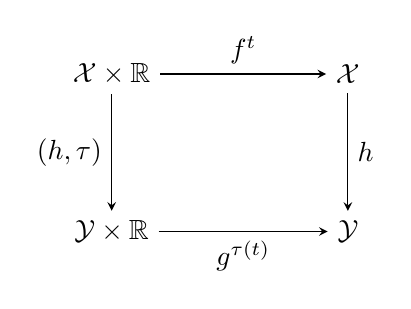
\begin{tikzpicture}[>=stealth, every node/.style={draw=none}]
  % Nodes
  \node (X1) at (0, 2) {$\mathcal{X} \times \mathbb{R}$};
  \node (X2) at (3, 2) {$\mathcal{X}$};
  \node (Y1) at (0, 0) {$\mathcal{Y} \times \mathbb{R}$};
  \node (Y2) at (3, 0) {$\mathcal{Y}$};

  % Arrows
  \draw[->] (X1) -- node[above] {$f^t$} (X2);
  \draw[->] (X1) -- node[left] {$(h,\tau)$} (Y1);
  \draw[->] (X2) -- node[right] {$h$} (Y2);
  \draw[->] (Y1) -- node[below] {$g^{\tau(t)}$} (Y2);
\end{tikzpicture}
\end{center}
Having this foundation allows us to more precisely describe the geometry of the dynamical system. First up, we shall see that the dynamical system has a very particular structure locally around stationary points. Stationary points serve a parallel purpose to those defined in introductory calculus. For us, we will understand them as follows:
\begin{mydefinition}{Stationary Points}
Let $F:\mathcal{X}\to \mR^d$ be a $C^1$ vector field with $\mathcal{X}\subset \mR^d$ open. We say that
\begin{itemize}
	\item $p\in \mathcal{X}$ is \emph{stationary} if $F(p)=0$,
	\item a stationary point $p\in \mathcal{X}$ is \emph{simple} if the Jacobian $DF(p)$ has full rank,
	\item a simple stationary point $p\in \mathcal{X}$ is \emph{hyperbolic} if all the eigenvalues of $DF(p)$ have non-zero real parts,
	\item a hyperbolic stationary point is an \emph{attractor} if all eigenvalues of $DF(p)$ have negative real parts,
	\item a hyperbolic stationary point is a \emph{repeller} if all eigenvalues of $DF(p)$ have positive real parts, and
	\item a hyperbolic stationary point is a \emph{saddle point} if it is neither an attractor nor a repeller.	
\end{itemize}
\end{mydefinition}
It is straightforward to see that if $p$ is a stationary point of a $C^1$ vector field, then $p$ is a fixed point of the time $t$-maps of the dynamical system arising from the autonomous differential equation \ref{diffeqvf}, i.e. $f^t(p)=p$. Moreover, it is not too hard to show that $Df_p(t)=\exp(tDF(p))$ with $f_p$ the trajectory of $p$. This allows us to translate the properties in terms of the vector field into properties in terms of the flow. With this terminology settled, we will now look at how these definitions correspond to geometric properties of flows around stationary points. One classical result is the Grobman-Hartman theorem:
\begin{thm}[Grobman-Hartman Theorem for Flows]
Let $p\in \mathcal{X}$ be a hyperbolic stationary point of a $C^1$ vector field $F:\mathcal{X}\to\mR^d$. Then there exist neighborhoods $\mathcal{V}$ of $p$ and $\mathcal{W}$ of $0\in \mR^d$, and a topological conjugacy $H:\mathcal{V}\to\mathcal{W}$ with $H(p)=0$ conjugating the flow of $F$ restricted to $\mathcal{V}$ to the flow of the linear vector field $A=DF(p)$ restricted to $\mathcal{W}$.
\end{thm}
This theorem shows that we can linearize the flow around stationary points, which in turn gives way for a much richer description of the geometry of the flow. We find that that we can aptly describe this structure with the theory of manifolds. The key reasoning behind this result, is that the we can extrapolate behaviour around the fixed points of a flow from the linearization given by the Grobman-Hartman Theorem. We record all this structure in the following result, which is also the main result of this theoretical section and links the theory of dynamical systems with the theoretical results on state space reconstruction, we will consider in the rest of chapter. It goes as follows:
\begin{thm}[Stable Manifold Theorem]\label{stable}
Let $F:\mathcal{X}\to \mR^d$ be a $C^k$ vector field, $k\geqslant 1$, at let $p\in \mathcal{X}$ be a hyperbolic stationary point, and let $A:\mR^d\to\mR^d$ be the linear map $x\mapsto DF(p)x$. Moreover, let $(f^t)_t$ be the flow of $F$. Then there exists invariant subspaces $E^s,E^u\subset\mR^d$, satisfying that 
\begin{enumerate}[label=(\roman*)]
	\item $E^s,E^u$ decompose $\mR^d$: $\mR^d=E^s\oplus E^u$,
	\item $E^s,E^u$ are invariant under $A$: $A(E^s)\subset E^s$ and $A(E^u)\subset E^u$,
	\item all eigenvalues of a matrix representing $A|_{E^s}$ have negative real parts, and all eigenvalues of a matrix representing $A|_{E^u}$ have positive real parts.
\end{enumerate}
Moreover there exist injective $C^k$ maps $\psi^s: E^s\to \mathcal{X}$ and $\psi^u:E^u\to\mathcal{X}$ satisfying that
\begin{enumerate}[label=(\roman*)]
\setcounter{enumi}{3}
	\item $\psi^s(0)=\psi^u(0)=p$,
	\item $D\psi^s(0)E^s=E^s$ and  $D\psi^u(0)E^u=E^u$,
 \item $\psi^s,\psi^u$ are of maximal rank: for all $u\in E^s$, $$\rank D\psi^s(u)=\dim E^s$$ and for all $v\in E^u$, $$\rank D\psi^u(v)=\dim E^u,$$
 \item and the images of $E^s/E^u$ under $\psi^s/\psi^u$ are attracting/repelling:
 \begin{align*}
  \psi^s(E^s)&=\{x\in \mathcal{X}:\lim_{t\to\infty}f^t(x)=p\},\\
 \psi^u(E^u)&=\{x\in \mathcal{X}:\lim_{t\to\infty}f^{-t}(x)=p\}
 \end{align*}
\end{enumerate}
\end{thm}
This theorem implies that if we have reason to believe that we are observing trajectories from a dynamical system that converge to some steady state or limit, then the theorem above realizes that trajectory on a suitable set, that has a lot of structure. We will quickly see that these sets are in fact manifolds, as we are about to define. As for the proofs of the Grobman-Hartman theorem and the stable manifold theorem, we refer once more to \cite{Dynamics}. Before that, there are several important remarks to make to this theorem:
\begin{itemize}
	\item If $p$ is an attractor, then we see that $E^s$ is all of $\mR^d$, and if $p$ is a repeller, then $E^u$ is all of $\mR^d$. In particular, if $p$ is an attractor, we observe by the mere fact that $\mathcal{X}\subset \mR$ that the attractor set $\psi^s(E^s)$ is a neighbourhood of $p$, so everything around $p$ will converge to this point. 
	\item If $\mathcal{X}$ is compact and convex, then it is a consequence of Brouwer's fixed point theorem that a time $t$-map $f:\mathcal{X}\to\mathcal{X}$ has a fixed point $p\in \mathcal{X}$, and if it is hyperbolic this activates the stable manifold theorem. This is in fact a stronger statement than that of the stable manifold theorem, since it implies the latter by the correspondence between fixed points of time $t$-maps of a vector field and stationary points of the vector field.
	\item It is a generic property that a linear map $\mR^d\to\mR^d$ is hyperbolic, meaning that the set of hyperbolic linear vector fields is an open and dense set of the space $\mathcal{L}(\mR^d,\mR^d)$ equipped with any topology induced by a norm: for instance one could go the matrix representation and use the matrix norm. This is the first example of a generic property in this thesis, but we shall see that this a typical concept in this setting.
\end{itemize}
We see that the stable manifold theorem can be more eloquently formulating in the language of manifolds. In practice, the manifolds we will consider can always be thought of as subspaces of $\mR^d$ for a suitable dimension $d\in \mN$, but it does help somewhat in the eloquence and not much intuition is lost. To that end, we do some heavy lifting now in generalizing the basic concepts from calculus to the world of differential topology and manifolds in order to better formulate the theorems in subsequent sections:
\begin{mydefinition}{Manifolds}
Let $M$ be a separable Hausdorff space and let $m\in \mN$.\\[5pt]
We call $(U,h)$ a \emph{chart} if $U\subset M$ is open and $h: U\to \mR^m$ is a homeomorphism onto its range with $U$ the \emph{chart domain} and $h$ the \emph{coordinate function}.\\[5pt]
If for each point $x\in M$, there exists a chart $(U,h)$ on $M$ such that $x\in U$, we call $M$ a \emph{manifold of dimension $m$}, and we call a collection of charts whose chart domains cover all of $M$ an \emph{atlas}. The collection of all charts on $M$ is itself an atlas that we call the \emph{structure} on $M$.\\[5pt]
On overlapping chart domains of charts $(U,h)$ and $(V,g)$, we consider the \emph{coordinate transformations}
$$hg^{-1}: g(U\cap V)\to \mR^m, \text{ and } gh^{-1}: h(U\cap V)\to \mR^m$$
We say that $M$ is \emph{differentiable} if $hg^{-1}, gh^{-1}$ are differentiable, we say the charts are \emph{$C^r$-related} if the coordinate transformations $hg^{-1}, gh^{-1}$ are $C^r$, and if all coordinate transformations of an atlas are $C^r$-related, we say the atlas is \emph{$C^r$-differentiable}. A \emph{differential structure} is the set of all charts $C^r$-related to the charts in some atlas. We shall say a manifold is $C^r$ if there exists a $C^r$-differentiable atlas of $M$.\\[5pt]
If $M$ is $C^r$ and $N$ is a $C^r$ manifold of dimension $n\geqslant m$, the function $f: M\to N$ is \emph{$C^r$-differentiable} if for each $p\in M$, there exists charts $(U,h)$ on M and $(V,g)$ on N, such that $p\in U$, $f(p)\in V$ and 
$$gfh^{-1}: h(U\cap f^{-1}(V))\to \mR^n$$
is $C^r$. (Remark: this property thus holds for any choice of charts in the atlas covering $p$ and $f(p)$ respectively). The \emph{Jacobian} at $p$ is then defined as 
$$Dgfh^{-1}(h(p))$$
This depends on the choice of charts but the rank does not.\\[5pt]
If the Jacobian is of maximal rank (rank $m$), we say $f$ is \emph{immersive at p}, and if $f$ is immersive everywhere, then we say $f$ is an \emph{immersion}. An immersion that is homeomorphic upon its image is an \emph{embedding}.\\[5pt]
Conversely, if $m\geqslant n$, and the Jacobian is of maximal rank (rank $n$), then $f$ is \emph{submersive at $p$}, and if submersive everywhere it is a \emph{submersion}. If $f: M\to N$ is an embedding, we say that $f(M)$ is a \emph{submanifold} of $N$.\\[5pt]
A \emph{diffeomorphism} is a map $f:M\to N$ for which there exists a differentiable inverse, and in this case we shall call $M$ and $N$ \emph{diffeomorphic}. If $f$ is an embedding, it is possible to prove that $f:M\to f(M)$ is a diffeomorphism.\\[5pt]
The \emph{tangent space} to a differentiable manifold $M$ at the point $p\in M$ is the set, denoted $T_pM$, of the equivalence classes under the equivalence relation defined as follows: Let $\mathcal{C}(p)$ be the set of curves $c:I\to M$, $I\subset \mR$ an open set with $0\in I$, differentiable at $0$ and satisfying $c(0)=p$. We let $c_1\sim c_2$, if there exists a chart $(U,h)$ with $p\in U$ on $M$ such that $(h\circ c_1)'(0)=(h\circ c_2)'(0)$. We have the following local characterization on the chart $(U,h)$:
$$Dh(p):T_pM\to\mR^d,\quad [c]\mapsto (h\circ c)'(0)$$
\end{mydefinition}
\noindent We recognize immediately that the maps $\psi^s$ and $\psi^u$ of the stable manifold theorem (\ref{stable}) are injective $C^k$ immersions, and that the attractor and repeller sets $W^s(p)\coloneqq \psi^s(E^s)$ and $W^u(p)\coloneqq \psi^u(E^u)$ are indeed manifolds, that we usually call respectively the \emph{stable manifold} and the \emph{unstable manifold}. We recognize a certain likeness to the limiting distributions leading to undirected edges when working with chain graphs from the idea of attractor sets in the dynamical systems world. We end this section by extending the theory of dynamical systems to this manifold setting:
\begin{mydefinition}{Differential Equations on Manifolds}
A \emph{vector field} on a manifold $M$ is a map $F:M\to TM=\bigcup_{p\in M}T_pM$ with $F(p)\in T_p$, and a \emph{differential equation} on $M$ is given by
\begin{equation}\label{diffeqmanif}
x'(t)=F(x(t))
\end{equation}
meaning that for a chart $(U,h)$ on $M$, then
$$\forall x(t)\in U: (h\circ x)'(t)=Dh(F(x(t)))$$
with $x:\mR\to M$ a differentiable curve on $M$.
\end{mydefinition}
We solve differential equations on manifolds by localization on charts, using the results from theorem \ref{ThmDiffEq} to generate solutions. Of course some technicalities arise in this context, but it is mainly a matter of looking at the behavior on overlapping charts and using the properties of the coordinate transformations. In all essence, we can give the following analogy of theorem \ref{ThmDiffEq}:
\begin{thm}[Solutions to Differential Equations on Manifolds]\label{ThmManifDiffEq}
Let $M$ be a $C^1$-manifold of dimension $d$, and let $F:M\to TM$ be a $C^1$ vector field. Then
\begin{enumerate}[label=(\roman*)]
	\item for every $p\in M$, there exists a solution $x:I\to M$ to the equation \ref{diffeqmanif} with $0\in I$ and $x(0)=p$.
	\item if $x_1:I_1\to M$ and $x_2:I_2\to M$ are solutions to equation \ref{diffeqmanif} with $0\in I_1\cap I_2$ and $x_1(0)=x_2(0)$, then $x_1(t)=x_2(t)$ for all $t\in I_1\cap I_2$.
	\item The differential equation \ref{diffeqmanif} defines the flow $(f^t)_t$ with $f^t(p)=x(t)$ for all $p\in M$ and $x$ the unique solution going through $p$ at $0$.
\end{enumerate}

\end{thm}

\section{Takens' Theorem}
In the following, we will switch gears from the more welcoming realm of considering functions in $\mR^n$ and $\mR$ and move completely to the realm of differential topology, which is inhabited by manifolds, vector fields and tangent bundles as we have just defined. This is done, not for needless abstraction, but because the theory we shall be exploiting holds in this generality - and in fact as long as we consider compact manifolds, we might as well think of them in Euclidean spaces nonetheless. So in practice, we will always be able to envision our models living in our usual space $\mR^n$, but it is not in any way useful to restrict ourselves at this point.\\\\
We will consider different set-ups, but the base model is systems modelled as vector fields on invariant compact manifolds, which can be generalized to cover vector fields with an attractor set, that need not in fact be a manifold, see \cite{Sauer1991}. As the theorem itself, this is formulated in the realm of differential topology and so the objects involved in the theorem and subsequent theory spring from there. The fundamental result we shall use, now known as Takens' theorem, was proved in 1981 by Floris Takens, \cite{Takens}, and states that one can reconstruct the manifold using only a univariate observation function; that is observing only one variable over time allows us to reconstruct the entire path of the dynamic system of all variables. The original theorem as stated by Takens is as follows:
\begin{thm}[Takens' Theorem, Version 1]
Let M be a compact $C^2$ manifold of dimension $m$. For pairs $(\varphi,y)\in \text{Diff}^2(M)\times C^2(M,\mathbb{R})$, it is a generic property that the map $\Phi_{(\varphi,y)}:M\to \mathbb{R}^{2m+1}$, defined by
$$\Phi_{(\varphi,y)}(x)=(y(x),y(\varphi(x)),...,y(\varphi^{2m}(x))),$$
is an embedding. \cite{Takens}
\end{thm}
There are several things to unpack here. First of all, it is worth noting the differentiability constraints on our maps; both $\varphi: M\to M$ and $y:M\to\mR$ are required to be twice continuously differentiable. In the work of \cite{Sauer1991}, their setup enables this requirement to be relaxed to them only being once continuously differentiable. Next, we will call $y$ our \textit{observation function}, and we can think of this as what we observe from the system, and will take the place of random variables in this setting. The background space is now a dynamical system instead of a probability space, and the measurability   of a random variable translates to the differentiability of an observation function. For now, $\varphi$ is defined very generally, but we shall quickly make this map must more explicit as a time $t$-map.\\\\
We shall call $\Phi$ for the \textit{delay embedding}, the reasoning behind which will be revealed shortly. However, the most important caveat is perhaps that it is 'only' a generic property that the theorem yields a a reconstruction of the manifold, i.e. that the delay embedding actually is an embedding. By generic property is meant to be understood that for 'most' observation functions $y$ and most choices $\varphi$, the delay embedding is indeed an embedding and so this concept takes the place of almost surely from probability theory. The precise meaning in an algebraic sense is that there exists an open and dense subset of the function space $C^2(M,\mR)$, respectively $\text{Diff}^2$, for which the statement is true, when using the following topology:\\[5pt]
We let $C^r(M,N)$ denote the space of all $C^r$ differentiable maps from the $C^r$ manifold $M$ to the $C^r$ manifold $N$. We then let the topology of $C^r(M,N)$ be generated by the subbase consisting of sets defined as follows: for any choice of function $f\in C^r(M,N)$, charts $(U,h)$ on $M$ and $(V,g)$ on $N$, a compact set $K\subset U$ such that $f(K)\subset V$ and $\varepsilon>0$, we define $\mathcal{N}(f,(U,h),(V,g),K,\varepsilon)$ to be the set of all functions $\hat{f}\in C^r(M,N)$ for which $\hat{f}(K)\subset V$ and
$$\norm{D^kg\hat{f}h^{-1}(x)-D^kgfh^{-1}(x)}<\varepsilon$$
for all $x\in h(K)$, $k=0,\ldots,r$, where $\norm{\cdot}$ is the usual Euclidean norm. If $M$ and $N$ are diffeomorphic, we let $\text{Diff}^r(M,N)$ be the subspace of $C^r(M,N)$ consisting of $C^r$-differentiable diffeomorphisms equipped with the subspace topology. Usually, we will use the shorter $\text{Diff}^r(M)$ for $\text{Diff}^r(M,M)$.\\\\
From this stems our second regularity assumption. For $\varphi$, we will be able to do some reasoning in practical cases, but for $y$ this will often be just another silent assumption. We shall be calling a map $y\in C^2(M,\mR)$, respectively $\varphi\in \text{Diff}^2(M)$, \textit{generic} if there exists $\varphi\in \text{Diff}^2(M)$, respectively $y\in C^2(M,\mR)$, such that the resulting delay embedding is indeed an embedding.
We will now work towards a more explicit version of the theorem. First of all, the reasoning behind the naming of the delay embedding, comes from the following: we shall associate any given time point $t\in \mR_{\geqslant 0}$ with a position $x(t)\in M$ on the manifold. For a given delay length $\tau\in \mR_{>0}$, we may then define $\varphi_\tau: M\to M$ by $x(t)\mapsto x(t-\tau)$. This links this theorem to the dynamical systems, since these are exactly $-\tau$-time maps of the dynamical system. Substituting this into Takens' theorem reduces the delay embedding to
$$\Phi(x(t))=(y(x(t)),y(x(t-\tau)),\ldots,y(x(t-2m\tau)))$$
Takens' theorem thus states that the values of a single time series considered at different delays will reconstruct the manifold 'generically'. Now we will need to ensure that this choice of $\varphi$ is both twice continuously differentiable and is not of such a nature that it falls out of the set of generic functions. The differentiability constraint falls under the umbrella of regularity assumptions and is fulfilled for flows arising from autonomous differential equations of $C^2$ vector fields. Furthermore, we can guarantee that $\varphi^\tau$ will be generic for some choices of $\tau$ by the power of a restatement of Takens' theorem. It was in fact proved by Takens in \cite{Takens}, but not stated. We will follow the restatement of the theorem as well as the subsequent presentation of theory and definitions presented in \cite{Huke} for the rest of this section. We present the updated version of Takens' theorem:
\begin{thm}[Takens' Theorem, Version 2]\label{v2}
Let M be a compact $C^2$ manifold of dimension $m$. Let $\varphi\in\text{Diff}^2(M)$ satisfy
\begin{enumerate}[label=\arabic*)]
	\item the periodic points of $\varphi$ with periods less than or equal to $2m+1$ are finite in number,
	\item if $x$ is any such periodic point with period $k\leqslant 2m$, then the eigenvalues of $\varphi^k$ at $x$ are all distinct.
\end{enumerate}
 Then it is a generic property for $y\in C^2(M,\mR)$ that the map $\Phi_{(\varphi,y)}:M\to \mathbb{R}^{2m+1}$, defined by
$$\Phi_{(\varphi,y)}(x)=(y(x),y(\varphi(x)),...,y(\varphi^{2m}(x))),$$
is an embedding. \cite{Huke}
\end{thm}

By periodic with period less than or equal to $2m$, we mean that $\varphi^{k}(x)=x$ for some $k\leqslant 2m$. The proof of the theorem is quite involved and a thorough treatment of the technicalities and details is perhaps worthy of a thesis of its own. We will still outline the proof to illuminate the machinery of this theory. In the following, we will use the subspace topology on $C^2(M,\mR)$ inherited from $C^1(M,\mR)$ and likewise on $\text{Diff}^2(M)$. In all topological statements below, this is what is meant. The proof of the 2nd version of Takens' theorem runs in the following stages:
\begin{enumerate}[label=\roman*)]
	\item First we prove that the set of generic observation functions is open, and we basically just exploit the following standard fact in differential topology:
	\begin{thm}\label{tool}
	Let $M$ be a compact manifold, and let $N$ be any manifold. For $K\subset M$ a compact subset of $M$, the set of $C^r$ maps from $M$ to $N$ immersive on $K$ is open in $C^r(M,N)$. Moreover, the set of $C^r$ embeddings of $M$ in $N$ is open in $C^r(M,N)$. \cite{hirsch}
	\end{thm}
	Proving that the map $\mathcal{F}^2: C^2(M,\mR)\to C^2(M,\mR^{2m+1})$, defined by $$y\mapsto (y,y\circ\varphi,\ldots, y\circ \varphi^{2m}),$$ 
	is continuous then immediately proves that the set of generic observation functions is open in $C^2(M,\mR)$. This is done in the following familiar set of steps: one proves $F: C^2(M,\mR)\to C^2(M,\mR)$ defined by $y\mapsto y\circ\varphi$, for $\varphi\in \text{Diff}^2(M)$, is in fact continuous.  This is simply a matter of unravelling the definition of the topology above, and requires only a slight bit of trickery. We skip the details of these derivations. By induction, it follows that $F_n:  C^2(M,\mR)\to C^2(M,\mR)$ defined by $y\mapsto y\circ\varphi^n$ is in fact continuous.  The final detail is to use that the product topology of $C^r(M,\mR)^{2m+1}$ coincides with that of $C^r(M,\mR^{2m+1})$. Worth remarking here is that we have made no assumptions on $\varphi$ yet, any embedding will do. Likewise, we have not used $m$ to do anything yet. 
\end{enumerate}
The rest of the stages is about proving that the set of generic observation functions is also dense. We start this process by picking any observation function $y$ and any neighbourhood $\mathcal{N}$ of our observation function. We then proceed to locate a generic observation function within this neighbourhood by iteratively adjusting the observation function to ensure the resulting delay embedding satisfies one more criterion for an embedding. In this pursuit, we will frequently use theorem \ref{tool} and the following technical fact: If $y\in C^2(M,\mR)$, and $\psi_i\in C^2(M,\mR)$, $i=1,\ldots,N$ for some $N\in \mN$. Then for every neighbourhood $\mathcal{N}$ of $y$, there exists $\delta$ such that
\begin{equation}\label{tool2}
\forall a=(a_1,\ldots,a_n),\norm{a}< \delta: y+\sum_{i=1}^N a_i\psi_i\in \mathcal{N}
\end{equation}
Proving this is only a matter of exploiting the compactness of $M$ and using the definition of the topology on our function space. We proceed as follows:
\begin{enumerate}[label=\roman*)]
	\setcounter{enumi}{1}
	\item The next step is locating an immersion on the set of points with period less than or equal to $2m$, let us denote it $P_{2m}$. In this stage, we use our assumptions on $P_{2m}$: Since $|P_{2m}|<\infty$, we know by the Hausdorff property of $M$, that we can find pairwise disjoint neighbourhoods of the elements in $P_{2m}$, and thus separate the different elements of $2m$. Now by a fairly standard construction, we can for any point and two nested neighbourhoods of it assume the existence of a 'bump functiom', i.e. a $C^2$ function taking a positive value in the point, having derivative 0 in the smaller neighbourhood and being 0 outside the larger neighbourhood. This allows us to manipulate each of these points separately. Using that the eigenvalues of $\varphi^k$ at each point are all distinct, we can manipulate the Jacobian of $\Phi_{\varphi,y}$ by means of the chain rule and pushing $y$ around with \ref{tool2} ensuring that it has full rank. The considerations in \ref{tool2} allows us to do this iteratively: if we find an immersion $y'$ of some subset $A\subset P_{2m}$, then we can find a neighborhood contained in $\mathcal{N}$ containing $y'$ where all elements are immersions of $A$. This is true by theorem \ref{tool} and stage i), since the set of such immersions is open. After carefully handling this manipulation in each step, we can guarantee the existence of an immersion $y'$ on $P_{2m}$ inside $\mathcal{N}$.
	\item The next stage is to extend this procedure to an immersion on all of $M$. In this stage, we use the dimension of $m$: First we note, that by the inverse function theorem, $y'$ is an embedding of a neighbourhood of each point $p\in P_{2m}$ and thus an immersion of that neighbourhood. We then proceed to cover $M$ with charts:  We choose charts containing an element $p\in P_{2m}$ small enough to ensure that $y'$ is an immersion of its closure, and for an element $p\notin P_{2m}$, we have $p,\varphi(p),\ldots, \varphi^{2m}(p)$ are distinct, and thus we can choose a chart $U_p$ of $p$ such that $U_p,\varphi(U_p),\ldots, \varphi^{2m}(U_p)$ are disjoint. Furthermore, in each set we move to a smaller chart whose closure is contained in the larger chart. By compactness of $M$, this cover can be thinned to a finite number of charts. In this stage, our map is then iteratively extended to an immersion on the closure of such a chart not immersed already. Using a bump function on each chart and its image under $\varphi,\ldots,\varphi^k$ allows us once again to manipulate the Jacobian of $\Phi_{(\varphi,y)}$ by allowing us to push  each coordinate separately using \ref{tool2}. Using a standard argument, we can show that if the $s+1$'th column of the Jacobian is not linearly independent of the first $s$ linearly independent columns at any element of the chart, then this parametrizes a subspace of dimension $s+m$ of $\mR^{2m+1}$ for values of $a$.  The complement of this subspace is naturally open and dense, and thus we can find an element of any norm for which all columns are independent. This argument is in fact valid for only $2m$ coordinates of $\Phi$, we only need $2m+1$ for injectivity. Nonetheless, this identifies a perturbed observation function immersive on the closure of the entire chart - and by theorem \ref{tool} and stage i), this can be done iteratively to find $y''\in \mathcal{N}$ immersive on all of $M$.
	\item The final stage of the proof of the 2nd version is to establish injectivity. By the Inverse Function Theorem, this is true locally, so we just have to ensure this holds globally as well. This is by far the most technical part of the proof. Proving that there exists $y'''\in \mathcal{N}$ such that $\Phi_{(\varphi,y''')}(x)\neq \Phi_{(\varphi, y''')}(\varphi^j(x))$ unless $x=\varphi^j(x)$ can be achieved with a similar construction as in iii) separating charts, on which $\Phi_{(\\varphi,y'')}$ is an embedding, such that the images under $\varphi^j$, $j=0,\ldots,m$, are disjoint and then thinning to a finite number of charts before adjusting. Since $\Phi_{(\varphi,y''')}$ is injective in small neighbourhoods around all points in $M$, we then have for any $x,x'\in M$, $x\neq x'$, that if $\varphi^i(x)$ and $\varphi^j(x)$ land in the same small neighbourhood for say $i,j\leqslant 2m$, then $\Phi_{(\varphi,y''')}(x)\neq \Phi _{(\varphi,y''')}(x')$. Thus being able to separate orbits close to each other, allows us to look at the subset of $M\times M$ where this phenomenon does not happen. Identifying once more a reasonable cover of charts of $M$ well-behaved under $\varphi$, one can choose a partition of unity subordinate to this cover, that is a map for each chart that is zero outside the chart such that the sum of all functions in each point is 1. Looking then at \ref{tool2} where we name the element $y_{\varepsilon}$ of the pertubation of $y'''$ with the $\psi$-functions the partitions of unity and coefficients $\varepsilon_1,\ldots,\varepsilon_N$. We need to show that these coefficients can be chosen such that $\Phi$ becomes injective while still being sufficiently small. This is done by checking the image of $\Psi:M\times M\times \mR^N\to\mR^{2m+1}$ given by
	$$\Psi(x,x',\varepsilon_1,\ldots,\varepsilon_N)=\Phi_{(\varphi,y_{\varepsilon}})(x)-\Phi_{(\varphi,y_{\varepsilon}})(x')$$
	We will not spend more time on this part of the proof, but this is the part where it becomes crucial to go to $\mR^{2m+1}$ and not $\mR^{2m}$ since the dimension of the domain of $\Psi$ is $2m+N$, and we need $\Psi|_{X}^{-1}(0)$ to be of lower dimension than $N$. This is what allows us to choose $\varepsilon$'s to satisfy the constraint and yield an embedding. 
	\item The final stage is proving the 1st version of Takens' theorem from the 2nd version. It relies almost entirely on the the Kupka-Smale theorem:
	\begin{thm}[Kupka-Smale Theorem]
	If $M$ is a compact manifold, and $\varphi\in \text{Diff}^2(M)$, then it is a generic property that for some integer $n\in \mN$, that the number of periodic points with period $n$ or less is finite.
	\end{thm}
	There is a little in work in showing that one can extend this when incorporating the second condition of the 2nd version, and one also needs to use an argument similar to that in stage i) to prove the openness claim in the function space $\text{Diff}^2(M)\times C^2(M,\mR)$ instead of just in $C^2(M,\mR)$. But in essence, it is the Kupka-Smale theorem that links the two theorems.
\end{enumerate}  
The theorem warrants a few comments. First, we see that in general we need to deal with periodic points quite explicitly. If we don't expect periodic points, then we come far quite quickly. And moreover, when working with flows the time lag could be varied a bit to yield a generic function. In principle, multiple lags can be tested, and we should thus be able to sidestep this problem. \\[5pt]
In contrast to the choice of $\tau$, we will have less flexibility in the choice of observation functions. So even if the same technique of small perturbations of a non-generic observation function produces a generic observation, we do not have access to it. Therefore we will usually have to assume a given observation function is generic, if there is no reason to believe otherwise. However, in some cases we can actually endow genericity with causal interpretation - we return to this in the next section.\\[5pt]
Even though Takens' theorem itself might appear somewhat magical, it should actually not be seen as too big of a surprise. As noted above, a property being generic is very analogous to an identity holding almost surely in probability theory. One problem is that the space of all differentiable functions is usually an infinite-dimensional space, which implies that a generalization of the Lebesgue measure to such a space is not straight-forward. However, it is possible to link the two concepts. To this end, we introduce the concept of prevalence:
\begin{mydefinition}{Prevalence}
Let $V$ be a normed vector space over $\mR$.\\[5pt]
The $\sigma$-algebra $\mathcal{B}$ generated by all open sets in $V$ is called the \emph{Borel $\sigma$-algebra on V} and $S\in \mathcal{B}$ is called a \emph{Borel subset of $V$}. If $V$ is finite-dimensional of dimension $d$, $V\cong \mR^d$ in the sense of isometry and this map defines a (unique) Lebesgue measure $\lambda $on $V$.\\[5pt]
We say that a Borel subset $S\subset V$ is \emph{prevalent} if there is a finite-dimensional subspace $E$ of $V$ such that for each $v\in V$, we have $v+e\in S$ for Lebesgue almost every $e\in E$, i.e.
$$\lambda_E\left(\left\{e\in E\mid v+e\notin S\right\}\right)=0$$
We then call $E$ a \emph{probe space of $S$}.\\[5pt]
If $S$ is a prevalent subset of $V$, then we say that $v\in S$ for \emph{almost every $v\in V$}.
\end{mydefinition}
We see that a prevalent set satisfies that if we start at any point in the ambient space $V$, then any exploration according to the directions of the finite-dimensional probe space will end in $S$ almost surely. This captures the essence of $S$ inhabiting 'most of' $V$ in the 'directions of $E$'. This becomes immediately more appealing, once we realize that this is much more all-encompassing than what it seems at first glance: Assume that $E'\subset V$ is a finite-dimensional subspace containing a probe space $E$ of $V$. Let $v_1,\ldots,v_n$ be an orthonormal basis of $E'$, such that $v_1,\ldots,v_k$, $k<n$, spans $E$. By Fubini's theorem, we then realize
\begin{align*}
\lambda_{E'}\left(\left\{e'\in E':v+e\not\in S\right\}\right)&=\int 1_{\{e'\in E'\mid v\in e'\notin S\}}\ d\lambda_{E'}\\
&=\int\int 1_{\{e'\in E'\mid  v\in e'\notin S\}}\ d\lambda_{E}\ d\lambda_{\langle v_{k+1},\ldots, v_n \rangle}\\
&=0
\end{align*}
This means that we can arbitrarily extend a probe space, and so $S$ is really 'everywhere' in $V$ if $S$ is prevalent. This motivates the definition of 'almost every' as an extension of almost surely. Indeed, when $V$ is finite dimensional we recognize that the complement of a prevalent set has measure 0. This concept of prevalence is not one-to-one with the concept of genericity, but allows for similar embedding theorems. Quite importantly, we can formulate Takens' theorem with this concept instead:
\begin{thm}[Takens' Theorem, Version 3]
Let M be a compact $C^1$ manifold of dimension $m$. Let $\varphi\in\text{Diff}^1(M)$ satisfy
\begin{enumerate}[label=\arabic*)]
	\item the periodic points of $\varphi$ with periods less than or equal to $2m+1$ are finite in number,
	\item if $x$ is any such periodic point with period $k\leqslant 2m$, then the eigenvalues of $\varphi^k$ at $x$ are all distinct.
\end{enumerate}
 Then for almost every $y\in C^1(M,\mR)$, the map $\Phi_{(\varphi,y)}:M\to \mathbb{R}^{2m+1}$ defined by
$$\Phi_{(\varphi,y)}(x)=(y(x),y(\varphi(x)),...,y(\varphi^{2m}(x))),$$
is an embedding. \cite{Sauer1991}
\end{thm}
We see this relaxes the $C^2$ assumption, but is otherwise identical. In fact, it turns out that Takens' embedding theorem is only a particular result of a quite general phenomenon. This is made explicit in a result of \cite{Sauer1991}, that restates the Whitney embedding theorem in the following way:
\begin{thm}[Whitney Embedding Prevalence Theorem]
Let $M$ be a compact $C^1$ manifold of dimension $d$. Almost every $C^1$ map $M\to \mR^{d+1}$ is an embedding of $M$.
\end{thm}
This shows that in reality, it is more a feature of manifolds than any special structure of the delay embedding, that allows us to reconstruct a manifold. The relevance of Takens' theorem thus stems more from its practicality compared to its  theoretical implications on the existence of embeddings. When working with time series, the delay map is a very natural construction and Takens' theorem gives theoretical backing on its usability. We end this section by stating a generalization of Takens' theorem proved in \cite{Sauer1991}. We need a little bit of additional terminology:
\begin{mydefinition}{Box-Counting Dimension}
Let $A\subset \mR^n$ be a compact set. Let $\norm{x}_{\infty}=\max_ i |x_i|$ for $x=(x_1,\ldots,x_n)\in \mR^n$. We then say that $B$ is a \emph{box} of length $\varepsilon>0$ if there exists $x_0\in \mR^n$ such that $$B=\{x\in \mR^n\mid \norm{x-x_0}_{\infty}\leqslant \varepsilon \}$$
Let then $N(\varepsilon)$ be the minimum number $N$, satisfying that there exists $N$ boxes $B_1,\ldots,B_N$ of length $\varepsilon$ such that
$$A\subset \bigcup_{m\in\{1,\ldots,N\}} B_m$$
If $-\log(\varepsilon)^{-1}\log N(\varepsilon)$
converges as $\varepsilon \to 0$, then we define the \emph{box-counting dimension} or the \emph{Minkowski-Bouligand dimension} as
$$\dim_{\text{box}}\coloneqq \lim_{\varepsilon\to 0}\frac{\log N(\varepsilon)}{\log(1/\varepsilon)}$$
\end{mydefinition}
It takes quite a bit of work, but it is possible as a reality check to show that a manifold of dimension $d$ has box-counting dimension $d$, so this dimension is consistent with the natural one on manifolds. In general, the box-counting dimension is very useful when working with fractals and sets of which we do not require a significant amount of structure. However, it turns out that it is all we need. For more details on this construction, we refer to \cite{Fractals}. This allows for the following generalization of Takens' theorem in the prevalence theorem of \cite{Sauer1991}:
\begin{thm}[Takens' Theorem, Version 4]
Let $U\subset \mR^k$ be open, let $A\subset U$ be a compact subset of $U$ with $\dim_\text{box}(A)=d$ and let $n>2d$ be an integer. If $\varphi\in\text{Diff}^1(U)$ and
\begin{enumerate}[label=\arabic*)]
	\item for every positive integer $p\leqslant n$, the set $A_p$ of periodic points of period $p$, i.e.
	$$A_p\coloneqq \left\{a\in A\mid \varphi^p(a)=a\right\}$$
	satisfies $\dim_\text{box}(A)<p/2$,
	\item if $a$ is any such periodic point with period $p\leqslant n$, then the eigenvalues of $\varphi^p$ at $a$ are all distinct.
\end{enumerate}
or if $(\varphi^t)_{t\in \mR}$ is a $C^1$ flow on U with $\varphi=\varphi^1$ and satisfy
\begin{enumerate}[label=\arabic*)]
	\item $A$ contains a finite number of equilibria, i.e.
	$$\abs{\left\{a\in A\mid \forall
	 t\in \mR: \varphi^t(a)=a\right\}}<\infty$$
	 \item there are no periodic points of period $1$ or $2$ of $\varphi$,
	\item for every positive integer $p\leqslant n$, the set $A_p$ of periodic points of period $p$ of $\varphi$ is finite,
	\item if $a$ is any such periodic point with period $p\leqslant n$, then the eigenvalues of $\varphi^p$ at $a$ are all distinct.
\end{enumerate}
then for almost every $y\in C^1(U,\mR)$, the map $\Phi_{(\varphi,y)}:M\to \mathbb{R}^{2m+1}$ defined by
$$\Phi_{(\varphi,y)}(x)=(y(x),y(\varphi(x)),...,y(\varphi^{2m}(x))),$$
is
\begin{enumerate}[label=\roman*)]
	\item injective on $A$,
	\item an immersion on each compact subset $C$ of a $C^1$ manifold contained in $A$.
\end{enumerate}
\end{thm} 
This yields a link with the stable manifold theorem, in that the stable manifold theorem shows us that manifolds arise around equilibriums in the attracting and repelling sets, and this theorem then establishes an embedding of these manifolds on compact subsets. With this settled, we move to modelling causality in a dynamical setting.

\section{Causal Inference with Takens' Theorem}
In this section, we will exploit Takens' theorem for inference of a graph structure of a model. We define a dynamical system according to a graph structure to mirror the structural causal model:

\begin{mydefinition}{Structural Dynamic Causal Model}
A \emph{structural causal dynamic model (SDCM)} $\mathfrak{O}$ over a set of deterministic time series $(X_v)_\mathcal{V}\in \mR^\mathcal{V}$ with respect to a DAG $\mathcal{G}=(\mathcal{V},\mathcal{E})$ consists of a collection of deterministic functions $(f_v)_{v\in \mathcal{V}}$ satisfying that
\begin{itemize}
	\item the function $f_v$ depends on $\left(x_v,x_{\pa(v)} \right)$,
	\item each variable satisfies
	$$ X_v'(t)=f_v\left(\left(X_v,X_{\pa(v)}\right)(t)\right)$$
	\item the intervention 
	$$X_a'
	(t)\coloneqq q\left(X_a,X_{\pa'(a)}\right)$$ 
	for $a\in \mathcal{V}$ with respect to the DAG $\mathcal{G}'$ differing only from $\mathcal{G}$ by the parents of $a$, induces the \emph{postintervention SOM} with respect to $\mathcal{G}'$ obtained by replacing $f_a$ with $q$.
\end{itemize}
If $u\in \pa(v)$ for $u,v\in \mathcal{V}$, we call $X_u$ the \emph{cause} and $X_v$ the \emph{effect}. 
\end{mydefinition}
This definition runs parallel the definition of \emph{kinetic causal modes} in the work of \cite{KCM}, although our definition is slightly more general. The definition is heavily motivated by the SCM; compared to the multivariate SCM this differs due to the time dependence, which replaces the noise terms as the source of variability in the model. We expect time- and space-homogeneity here - namely that the 'update rule' is consistent across time and space of the model. The space-homogeneity is shared with the multivariate SCM, where the assignment functions are not allowed to depend on the outcome of the noise variables, while the time-homogeneity is built-in with the time series SCM. We do allow for lags in this model specification - so the model does not allow for memory of the past to influence the update rule of the system. This is reminiscent of a Markov property in this setting.\\[5pt]
We could try to circumvent this problem, for instance by including a derivative as a variable or a lagged variable, but seeing as the relationship between a variable and its lagged version is not expressible with the functions of the SOM, it is not possible to model this directly with the framework above. We will try to accomodate this at the end of the section. It is however possible to model the relationship between a variable and its derivative, so this is doable, but requires care when considering interventions - it does not really make sense to intervene on the link between a variable and a derivative.\\[5pt]
What we can do, is prove an equivalent of theorem \ref{entail} for SOMs guaranteeing a resulting flow satisfying a decomposition property according to the graph. The idea is to replace the object of interest from distribution to flow, and the Markov property to one that decomposes the flow instead of the density. As we have already seen, we can construct a flow from a differential equation as the one resulting from an SOM, and theorem \ref{ThmDiffEq} gives sufficient conditions for it to be complete and unique in terms of the update functions. The Markov property is replaced by the following property:
\begin{prop}
Given an SOM $\mathcal{D}$ over $\mathcal{G}=(\mathcal{V},\mathcal{E})$, and ancestral sets $U,V\subset \an(\mathcal{G})$ with $U\subset V$, the family of maps $\{\varphi^t_W\}_{W\in \an(\mathcal{G})}$, where $\varphi_U^t$ is defined on $\mR_U$ and given by the equation
$$\varphi^t_U\circ\pi_U(x)=\pi_U\circ \varphi^t(x)$$
for all $x\in \mR$, is well-defined, and the the collection $(\mR_U,\pi_{UV})_{d}$ of dynamical systems is consistent, meaning that they satisfy
$$\pi_{VU}\circ \varphi_V^t(x)=\varphi_U^t(x)\circ\pi_{VU}(x)$$
for all $x\in \mR_V$.
\end{prop}
\begin{proof}
Suppose $\pi_U(x)=\pi_U(y)$ for $x,y\in \mR^n$. Hence $x,y$ differ in the variables $|\mathcal{V}_\varphi|\setminus |U|$, and since $U$ is an ancestral set, it follows that $\pi_U(\phi^t(x))=\pi_U(\phi^t(y))$, since the values of $\varphi^t$ on the variable set $|U|$ does not depend on the variables  among $|\mathcal{V}_\varphi|\setminus |U|$.\\
Observe that since each $x\in \mR_V$ can be written as $\pi_V(x')$ for some $x'\in \mR$, and since we can rewrite
\begin{align*}
\pi_U\circ\varphi^t(x')
&=\varphi_U^t(x)\circ\pi_U(x')=
\varphi_U^t\circ\pi_{VU}\circ\pi_V(x')=\varphi_U^t\circ\pi_{VU}(x),\quad\quad \text{and}\\
\pi_U\circ\varphi^t(x')&=\pi_{VU}\circ \pi_V\circ\varphi^t(x')=\pi_{VU}\circ \varphi_V^t\circ \pi_V(x')=\pi_{VU}\circ\varphi_V^t(x)
\end{align*}
by consistency of the projection mappings, we get consistency of the collection as desired.
\end{proof}
We will record this property as a definition in its own right, since it is instrumental in recovering some of the graph structure with Takens' theorem:
\begin{mydefinition}{Takens Property}
We say a flow $(\varphi^t)_{t\in \mR}$ satisfy \emph{Takens property} with respect to a graph $\mathcal{G}=(\mathcal{V},\mathcal{E})$ if there for every ancestral set $U$ exists a projection $\pi_{U}$ (surjective, continuous) such that there exists a unique flow $\varphi^t_U$ satisfying
$$\varphi^t_{U}\circ \pi_{\mathcal{V}U}(x)=\pi_{\mathcal{V}U}\circ \varphi^t(x)$$
and further, if there for every two ancestral sets $U,V$ with $U\subset V$ exists a projection $\pi_{VU}$ (surjective, continuous) such that
$$\pi_{VU}\circ\varphi_V^t(x)=\varphi_U^t\circ \pi_{VU}(x)$$
\end{mydefinition}
With the theory that we have developed, the following result is immediate:
\begin{thm}[Entailed Flows from SOMs]
Every SOM $\mathfrak{O}$ induces a flow on $\mR^{\mathcal{V}}$ satisfying the Takens property. If the update functions are globally Lipschitz, then the flow is complete and unique.
\end{thm}
To use Takens' theorem, we need the state spaces of the flows to be well-behaved. The following proposition show that if the entire system has a nice phase space, then so does the flows on each subsystem:
\begin{prop}
Let $\varphi$ be a flow on some compact invariant set $A$ satisfying the Takens property. Then $A_U=\pi_U(A)$ is a compact invariant set under $\varphi_U$.\\[5pt]
If further, $A$ satisfies that there exists an open set $\mathcal{O}\supset A$ of initial conditions, such that $\varphi^t(o)\to A$ as $t\in \infty$ for $o\in \mathcal{O}$, then $\mathcal{O}_U\coloneqq \pi_U(\mathcal{O})$ satisfies that $\varphi^t_U(o)\to A_U$ as $t\in \infty$ for $o\in \mathcal{O}_U$.\\[5pt]
Finally, if further there exists no proper subset $B\subset A$ satisfying that there exists an open set $\mathcal{O}^B\supset B$ of initial conditions, such that $\varphi^t(o)\to B$ as $t\in \infty$ for $o\in \mathcal{O}^B$, then there exists no proper subset $B_U\subset A_U$ satisfying that there exists an open set $\mathcal{O}_U^B\supset B_U$ of initial conditions, such that $\varphi^t(o)\to B_U$ as $t\in \infty$ for $o\in \mathcal{O}^B_U$.
\end{prop}
This ensures that properties of a dynamical system satisfying the Takens property is automatically preserved when moving to the subflows induced by the graph. The proof is quite straight-forward, compactness is directly inherited by means of continuity, invariance by construction of the subflows $\pi_U$, and the remaining details on attraction is just a matter of unpacking continuity - we skip the topological details. This means that the phase space itself decomposes consistently according to the graph when fulfilling the Takens property. In particular, we have for all ancestral sets $U,V$ with $U\subset V$ that there exists a surjective continuous map from the state space $A_V$ to $A_U$ - but it is not given that such a map does not exist in the opposite direction. This is the analogue of the concept of faithfulness - we don't want to infer additional decompositions or identifications of the flow of a dynamical system. More serious, if $U$ and $V$ are incomparable, meaning that $U\not\subset V, V\not\subset U$, then we might encounter that there actually exists a continuous surjection from $A_U$ to $A_V$ although this is not what is implied by the Takens property. This will hinder inference, and we will try to assume this away:
\begin{mydefinition}{Fully Resolved State Space}
We say that the state space $A$ of flow $\varphi$ is \emph{fully resolved} with respect to a graph $\mathcal{G}$ if the following two conditions are met:
\begin{enumerate}[label=\roman*)]
	\item If $U,V$ are ancestral sets, with $U\subset V$, then the projection 
	$$\pi_{VU}:A_V\to A_U$$
	is non-injective.
	\item If $U,V$ are ancestral sets, with $U\not\subset V, V\not\subset U$, then there exists no continuous surjections
	$f:A_U\to A_V$ or $g:A_V\to A_U$.
\end{enumerate}
\end{mydefinition}
Now a more pressing question, is whether Takens' theorem can actually be established when moving to the state space $A_U$ for an ancestral set $U$. First of all, we have to assume that the assumptions on the state space is once again fulfilled - for reasonable systems this is to be expected in the following sense: The stable manifold theorem holds also when moving to a subsystem not depending on the rest in the functional expression of the derivative. Since we have not been specific about the nature of the compact manifolds or attractor sets arising from our models, we will assume this problem away. It is however, inherently unrealistic: if we look at the solution to a one-dimensional stochastic differential equation, the state space of this function cannot reasonably be a compact smooth manifold - no such object exists in $\mR$. In general, the trajectories of a set of ordinary differential equations do not form a compact manifold, and thus it is even more of a stretch to assume that it can be decomposed into smaller compact manifolds. Since any graph contains a root node, we see that the problem is inescapable.\\[5pt]
Another problem is that we now need it to be a generic property that each subflow is generic, and this is not a priori clear from our construction. This is however possible in the manifold case, as is shown by \cite{mathFound}:
\begin{thm}[Genericity of Filtrations]
For a $C^1$ compact manifold $M$ of dimension $m$ satisfying that $M_U$ is a $C^1$ manifold of dimension $m_U$ for all ancestral sets $U$, then it is a generic property for $\varphi\in C^2(M,M)$ that for each ancestral set $U$: 
\begin{enumerate}[label=\arabic*)]
	\item the periodic points of $\varphi_U$ with periods less than or equal to $2m_U+1$ are finite in number,
	\item if $x$ is any such periodic point with period $k\leqslant 2m$, then the eigenvalues of $\varphi^k_U$ at $x$ are all distinct.
\end{enumerate}
\end{thm}
The proof is very technical and would take up significant space. We refer to their proof, and use the result as a marker - and it is useful that we do not have to make assumptions on this part. In the attractor setting, a similar statement is conjectured by \cite{mathFound}, but not proven as of yet as far as the author is aware. This theorem combined with Takens theorem \ref{v2}, yields that it is a generic property for observation functions to give us an embedding of the manifold $M_U$. Now this allows us to formulate the main theorem in the manifold setting:
\begin{thm}[Identifiability in dynamic systems]
Let $M$ be a $C^1$ compact manifold of dimension $m$, let $\varphi$ be a generic flow on $M$ satisfying the Takens property with respect to a graph $\mathcal{G}$. Asume further that $M_U$ is a $C^1$ manifold for each ancestral set $U$, and $M$ is fully resolved.\\[5pt]
Let now $U,V$ be ancestral sets, let $\varphi_1,\varphi_2$ be corresponding observation functions and let $M_i=\Phi_{\varphi^T,y_i,k_i}(M)$ be the reconstructions, where $k_1\geqslant 2n_U$ and $k_2\geqslant 2n_V$. It then holds that:
\begin{enumerate}[label=\roman*.]
	\item $U=V$ if and only if there exists a homeomorphism
	$$\Psi_{1,2}:M_1\to M_2$$
	\item $U<V$ if and only if there exists a continuous surjective, noninjective map
	$$\Pi_{1,2}:M_2\to M_1$$ 
\end{enumerate}
\end{thm}
\begin{proof}
We proceed in the following steps:
\begin{enumerate}[label=\roman*.]
	\item \textit{Forward direction}: If $U=V$, then $\Psi_{1,2}=\Phi_{\varphi^T,y_2,k_2}\circ \Phi_{\varphi^T,y_1,k_1}^{-1}$ is a diffeomorphism of $M_1$ on $M_2$.\\[5pt]
	\textit{Reverse direction}: Assume the existence of $\Psi_{1,2}$. Then
	$$\Phi_{\varphi^T,y_2,k_2}^{-1}\circ \Psi_{1,2} \circ \Phi_{\varphi^T,y_1,k_1}$$
	is a homeomorphism from $M_U$ to $M_V$. Since the manifold is fully resolved, this implies that either $U\subset V$ or $V\subset U$, and thus that $U=V$.
	\item \textit{Forward direction}: If $U<V$, then there exists $\pi_{VU}:M_V\to M_U$ since $M$ is fully resolved. Then
	$$\Pi_{2,1}=\Phi_{\varphi^T,y_1,k_1}^{-1}\circ\pi_{VU}\circ \Phi_{\varphi^T,y_2,k_2} $$ is a non-injective surjection of $M_2$ on $M_1$.\\[5pt]
	\textit{Reverse direction}: Assume the existence of $\Pi_{2,1}$. Then
	$$\Phi_{\varphi^T,y_1,k_1}^{-1} \circ\Pi_{VU}\circ  \Phi_{\varphi^T,y_2,k_2} $$
	is a non-injective surjective from $M_V$ to $M_U$. Since the manifold is fully resolved, this implies that $U\subset V$.
\end{enumerate}

\end{proof}
We have now proven that under conditions (I1)-(I4), it is actually possible to determine the causal directions in a dynamical system. The first condition is a regularity assumption that things are sufficiently well-behaved. We will give an alternative statement, where this condition is replaced, but in spirit this type of assumption is needed for any reconstruction to take place. It is the author's view that this is a reasonable assumption in most settings: although it might never actually be true that an observed system is restricted to a compact smooth manifold, we can think as we do in any kind of modelling as the imagined dynamic being a simplified representation of the system, and as far as the observed system behaves somewhat controlled locally, such a representation will probably be useful in capturing information about the system.\\\\ The second and third conditions are somewhat less reasonable in appearance; we are assuming the non-existence of mappings that if they existed would undermine the theoretical foundation of the theorem. This is undesirable. As is done in \cite{mathFound}, this is referred to the \textit{manifold being fully resolved}. An implied interpretation hereof is that it is simply matter of observing sufficient amounts of a data to separate different parts of the system - more on this later. This assumption is quite a standard one, and it is something that will appear in practical considerations nonetheless. A further comment on this, is that it corresponds somewhat to the faithfulness assumption often made when working with structural causal models.\\\\ The final assumption is entirely impossible to test as well, but we will interpret genericity in the same way as \textit{almost everywhere}, and assume that it is unlikely that we would ever get non-generic functions by accident. The almost everywhere interpretation is often a probabilistic one whereas this one is not, but as so often the difference is philosophical.\\\\
We have to in
\begin{cor}
Let $\varphi$ be an SCDM, and let $UL_\varphi$ be the corresponding lattice. Assume that assumptions I1)-I4) are fulfilled for all elements in $UL_\varphi$. Then the following algorithm recovers the transitive closure of the component graph $CG_\varphi$:
\begin{enumerate}[label=\roman*.]
	\item Let the set of variables be the set of vertices in a graph we will call \emph{RG}.
	\item For every variable $x$, build the reconstructed manifold $M_x\coloneqq \Phi	_{(\varphi^T,x,k)(M)}$.
	\item For every pair $x$ and $y$, draw an edge $x\to y$ if there exists a continuous surjection $f:M_x\to M_y$.
\end{enumerate}
\end{cor}
We remark the inherent simplicity of this approach as compared with Granger causality: in Granger causality, we have to account for all relevant information in order to allow for causal reasoning; here we need only consider the prints of the time series themselves. Of course, some potential problems may hide in our rather abstract set of assumptions I1)-I4). For instance, we cannot rule out a causal mirage due to synchronization: imagine a common causal confounder between two systems resulting in two heavily synchronized, but essentially 'independent' dynamic systems. This would result in erroneous causal interpretations, and so the problem of hidden confounders presents itself in this world as well. However, we would expect these mirages to occur only in the presence of heavy synchronization, so this potential undermining of causal inference may be less severe than in similar problems.\\\\ 
We used the term independent before, which of course is not to be interpreted in the probabilistic sense, as this is entirely meaningless in our setup; all our objects are deterministic, and they are all trivially independent in a probabilistic model. It is not quite true in a literal way either, since we assume that they are linked by a common cause; so all  that is meant that any further dynamic not imposed by the cause must be inherent to the subsystem and thus 'independent' of other subsystems.\\[5pt]
For completeness, we state the result in the attractor version as well, sensing that it might be less unrealistic when considering practical considerations.
\begin{thm}[Identifiability in Dynamic Systems on Attractors]
Let $\varphi$ be a flow on $\mR^n$. Assume that $A\subset \mR^n$ is compact, $\varphi^t(A)\subset A$ and satisfies that there exists an open set $\mathcal{O}\supset A$, such that $\varphi^{t}(o)\to A$ as $o\to\infty$. Assume further that $A$ is minimal, i.e. no subset of $A$ satisfies the same properties, that $\varphi$ satisfy Takens property and that $A$ is fully resolved.\\[5pt]
Let now $U,V$ be ancestral sets, let $\varphi_1,\varphi_2$ be corresponding observation functions and let $A_i=\Phi_{\varphi^T,y_i,k_i}(A)$ be the reconstructions, where $k_1\geqslant 2\dim_\text{box}(A_U)$ and $k_2\geqslant 2\dim_\text{box}(A_V)$. It then holds that:
\begin{enumerate}[label=\roman*.]
	\item $U=V$ if and only if there exists an injective map
	$$\Psi_{1,2}:A_1\to A_2$$
	that is a bijection from the union of all smooth manifolds embedded in $A_1$, $\bigcup M_1\subset A_1$, to the union of all smooth manifolds embedded in $A_1$, $\bigcup M_2\subset A_2$ and a homeomorphism when restricted to a compact subset of a smooth manifold embedded in $A_1$.
	\item $U<V$ if and only if there exists a noninjective map
	$$\Pi_{1,2}:A_2\to A_1$$ 
	that is a surjection from $\bigcup M_1\subset A_1$ to $\bigcup M_2\subset A_2$ and continuous when restricted to any compact subset of a smooth manifold embedded in $A_2$.
\end{enumerate}
\end{thm}
The proof is very similar to the one we already covered. Now by the stable manifold theorem, we know that for each point $a$ in an attractor $A$ of a dynamical system generated by an autonomous differential equation, there is a stable manifold embedded in $A$. Let us denote this manifold by $W(a)$. Strengthening the 'faithfulness' assumptions on an attractor to the following:
\begin{mydefinition}{Strongly Resolved Attractor}
The dynamical system ($A,\varphi$) has a \emph{strongly resolved attractor filtration with respect to $\mathcal{G}$} if the following two conditions are met:
\begin{enumerate}[label=\arabic*)]
	\item If $U$, $V$ are ancestral sets, and $U\subset V$, then a projection $\pi_{UV}:A_V\to A_U$ is non-injective on $\bigcup_b W_V(b)\subset A_V$ to $\bigcup_a W_U(a)\subset A_U$.
	\item If $U,V$ are ancestral sets and $U\not\subset V$, $V\not\subset U$, then there is no surjection $f:\bigcup_{a} W_U(a)\to\bigcup_b W_V(b)$ that is also continuous when restricted to any compact subset of $W_U(a)$ for some $a\in A_U$.
\end{enumerate}
\end{mydefinition}
This allows for the following procedure:
\begin{cor}
Let $\varphi$ be an SCDM, and let $UL_\varphi$ be the corresponding lattice. Assume that assumptions I1)-I4) are fulfilled for all elements in $UL_\varphi$. Then the following algorithm recovers the transitive closure of the component graph $CG_\varphi$:
\begin{enumerate}[label=\roman*.]
	\item Let the set of variables be the set of vertices in a graph we will call \emph{RG}.
	\item For every variable $x$, build the reconstructed attractor $A_x\coloneqq \Phi	_{(\varphi^T,x,k)(A)}$.
	\item For every pair $x$ and $y$, draw an edge $x\to y$ if there exists a surjection
	 $$f:\bigcup_a W_1(a) \to \bigcup_a W_2^u(b)$$ 
	 that is continuous on any $C\subset W_1(a)$.
\end{enumerate}
Then this will recuperate the transitive closure of $\mathcal{G}$.
\end{cor}
This is the extent to which we will follow this theoretical trail. It does indeed become quite complicated, and in the lack of more specific theoretical results, we have to assume a lot of structure away. Nonetheless, it does provide a fairly general framework in the presence of attractor sets. There is only on piece of the puzzle missing. Usually, we will not get access to realizations of many different starting conditions, but only one trajectory. This is problematic in principle: if we are trying to infer from reconstructed manifolds, then we have problems.\\[20pt]

\begin{mydefinition}{Graphical Dynamic Model}
A \emph{graphical dynamic model} $\mathfrak{D}$ in a phase space $\mathcal{X}$ over a set of observation functions $(X_v)_\mathcal{V}$ with respect to a DAG $\mathcal{G}=(\mathcal{V},\mathcal{E})$ consists of a collection of deterministic functions $(f_v)_{\tau\in \mathcal{V}}$ and a flow $(\varphi_t)_{t\in \mR}$, satisfying that
\begin{itemize}
	\item the function $f_v$ depends on $\left(x_v,x_{\pa(v)} \right)$,
	\item each variable satisfies
	$$\forall x\in \mathcal{X}:\left. \frac{d}{dt}X_v\left(\varphi^t\right)\right|_{t=0}=f_v\left(\left(X_v,X_{\pa(v)}\right)(x)\right)$$
	\item the intervention 
	$$\forall x\in \mathcal{X}: \left.\frac{d}{dt} X_a(\varphi^t(x))\right|_{t=0}\coloneqq q\left(X_a,X_{\pa'(a)}\right)$$ 
	for $a\in \mathcal{V}$ with respect to the DAG $\mathcal{G}'$ differing only from $\mathcal{G}$ by the parents of $a$ and the random variable $N'_a$ independent from $(N_v)_{v\in \mathcal{V}\setminus \{a\}}$, induces the \emph{postintervention SCM} with respect to $\mathcal{G}'$ obtained by replacing $f_a$ with $q$.
\end{itemize}
If $u\in \pa(v)$ for $u,v\in \mathcal{V}$, we call $X_u$ the \emph{cause} and $X_v$ the \emph{effect}. 
\end{mydefinition}

In this section, we will show that we can only hope to recover the component graph from data using Takens' theorem. We shall later discuss attempts to reason further about the causal structure, but the results below will show that without further assumptions, we cannot distinguish direct and indirect causal links.\\\\
The aim of this section is to show that under suitable regularity assumptions, we can create a correspondence between strongly connected components and sub-manifolds, and tha	t this correspondence is precisely fine-grained enough to allow us to determine whether any two variables belong to the same strongly connected component and further the direction of the causal link if they do not. To do this, we have to formalize this correspondence. First of all, as discussed the component graph $CG_\varphi$ is a directed acyclic graph, and so we can think of the graph structure as a partial order, where $x,y\in CG_\varphi$ satisfy $y\geqslant x$ if $y\to x$. Considering then the upper sets, we inherit an ordering of these, since they are exactly defined with respect to the partial order, and since we are dealing with sets, we can unproblematically consider the union and intersection of upper sets. This structure is that of a lattice:

\begin{defn}[Driver]
Given a dynamical system $\varphi$, and two variables $x$ and $y$ of $\varphi$, the variable $x$ \emph{directly drives} $y$ if the dynamics of $y$ directly depend on $x$, that is $y_{t+1}=g(x,\cdot)$ for discrete systems and $\dot{y}=g(x,\cdot)$ for continuous.
\end{defn}
\begin{defn}[Component graph]
A subset of vertices $W\subset V$ of the interaction graph is called a \emph{strongly connected component}, if for any $u,v\in W$ there exists a directed path from $u$ to $v$ and a directed path from $v$ to $u$. We define the \emph{component graph} as the graph obtained from the interaction graph by taking the set of strongly connected components $\mathcal{S}$ as the set of vertices, and letting there be a directed edge from $p\in \mathcal{S}$ to $q\in \mathcal{S}$ if there exists a $u\in p,v\in q$ such that there exists a directed path from $u$ to $v$.
\end{defn}
Note that being strongly connected defines an equivalence relation. The component graph will turn out to be very relevant in the following analysis.
It will turn out that each upper set corresponds to a self-contained dynamical system. The final component in our later analysis is the so-called \textit{transitive closure}:
\begin{defn}[Transitive closure]
Given a DAG $\mathcal{G}=(\mathcal{V},\mathcal{E})$, the \emph{transitive  closure of $\mathcal{G}$} is the graph obtained from $\mathcal{G}$ by taking the vertices $\mathcal{V}$ and include the edge between $u\in \mathcal{V}$ and $v\in \mathcal{V}$ if and only if there is a directed path from $u$ to $v$.
\end{defn}
The transitive closure of a causal graph encodes only the causal direction between variables but cannot distinguish between direct and indirect causal links. In other words, from the transitive closure you can infer all descendants of a given variable, but not the causal graph itself. It will turn out that this is exactly what we will be able to recover with the modelling framework based on Takens' theorem.\\[10pt]
\begin{defn}[Lattice]
A \emph{lattice} $L$ is a partially ordered set if for every two elements $a,b\in L$, there exists a least common upper bound, called a \emph{join}, denoted $a \vee b$ and a greatest common lower bound, called a \emph{meet}, denoted $a\wedge b$. Further, we require that if $a_1\leqslant a_2$ and $b_1\leqslant b_2$, then
$$a_1\wedge b_1\leqslant a_2\wedge b_2$$
and
$$a_1\vee b_1\leqslant a_2\vee b_2$$
We shall call $L$ \emph{distributive}, if
$$a\wedge(b\vee c)=(a\wedge b)\vee (b\wedge c)$$
\end{defn}
We see that we can think of the set of upper sets as a lattice when equipping it with unions and intersections. This lattice is going to be the index set for our subdivisions of manifolds, and so this will give us a natural way to think of the causal structure. We introduce the notion of a filtration:
\begin{defn}[Filtration]
Let $I$ be a partially ordered set, and let $(X_i)_{i\in I}$ be a collection of topological spaces and let further $(\iota_{ij})_{j\leqslant i}$ be a family of continuous maps $\iota_{ij}: X_i\to X_j$ satisfying the consistency constraint
$$\iota_{ik}=\iota_{ij}\circ \iota_{jk}$$
Then $(X_i,\iota_{ij})_I$ is an \emph{inverse system}, and we will also refer to it as a \emph{filtration}. An inverse system indexed by $I'$ obtained from $I$ by reversing all relations will be called a \emph{descending filtration} on $(X_i)_I$.
\end{defn}
This allows us to consider the causal structure as an object, and we can now use this object to create the correspondence discussed above. We will now define a descending filtration on the phase space. For this, we shall utilize that we can think of any compact finite dimensional manifold as a subspace of $\mR^n$ for suitable $n$, in fact this very fact is implied by Takens' theorem, and we shall think of the observed values as the coordinates of $\mR^n$. This reduces the generality of the approach somewhat, but it lends itself to interpretability and the modelling framework introduced in the beginning of this chapter. This leads us to the definition of a descending filtration of the phase space:
\begin{defn}[Upper set filtration]
Let $UL_\varphi$ be the lattice imposed by considering the upper sets of the component graph of a dynamical system $\varphi$. For $U\in UL_\varphi$, we define $|U|$ as the set of all variables contained the upper set $U$ and we will call it \textit{variable set} of $U$. Further, we let $\mR_U$ be the space spanned by $|U|$ of dimension $\#|U|$ and we call this the \textit{phase space} of $U$. We see now that for $U,V\in UL_\varphi$, we have $U\leqslant V$ if and only if $|U|\subset |V|$, which in turn is equivalent with $\mR_U\subset \mR_V$. We thus get a natural projection $\pi_{VU}:\mR_V\to\mR_U$. We further define $\pi_U$ as the natural projection $\mR^n\to \mR_U$. We see that this defines a descending filtration, and we call $(\mR_U,\pi_{UV})_{UL_\varphi}$ the \emph{upper set filtration of the phase space}.
\end{defn} 

This allows us to introduce a filtration of the manifolds on which our models live:
\begin{defn}
Let $\varphi$ be a dynamical system restricted to a compact invariant manifold. Then we will call the descending filtration $\{M_U\}_{U\in UL_\varphi}$, with $M_U$ defined by $M_U\coloneqq \pi_U(M)$, equipped with the family of maps $\pi_{VU}$, for the \emph{invariant set filtration} $\mathbb{M}$.
\end{defn}
We notice immediately that for any $U\in UL_\varphi$, then $M_U$ is a compact invariant set for the dynamical system $\varphi^t_U$. We can now decompose our dynamical systems into smaller dynamical systems based on the causal structure, and we now give a similar decomposition of the observation functions:
\begin{defn}[Filtration of observation functions]
For $U\in UL_\varphi$, let $Y_U\coloneqq C^2(M_U,\mR)$ denote the set of observation functions on $M_U$, and define $\iota_{UV}:Y_U\to Y_V$ by $\iota_UV(\varphi)=\varphi\circ \pi_{VU}:M_V\to \mR$. We call this the \emph{filtration of observation functions} and denote it $\mathbb{Y}$.
\end{defn}

\section{Ergodic Theory}
If we want to talk about the behaviour of a single trajectory in the state space, we have to introduce some ergodic theory. The anchor is the following definition:
\begin{mydefinition}{Invariant and Ergodic Measures}
If $f:X\to X$ is a homeomorphism, $\mu$ is an \emph{invariant $f$-measure} if for all $A\subset X$ $\mu(f(A))=\mu(A)$.\\[5pt]
An invariant measure $\mu$ is called \emph{ergodic with respect to $f$}, if it is true for all $f$-invariant sets $A\subset X$ that either $\mu(A)=0$ or $\mu(X\setminus A)=0$.\\[5pt]
We define the \emph{support} of a Borel measure $\mu$ as:
$$\supp \mu=\{x\in X\mid \mu(U)>0 \text{ for } x\in U, U \text{ open }\}$$
\end{mydefinition}
There are two key results of this theory that we record here:
\begin{thm}[Krylov-Bogolubov Theorem]
Any continuous map $f$ on a metrizable compact space has an ergodic invariant Borel probability measure.
\end{thm}
\begin{thm}[Birkhoff Ergodic Theorem]
Let $T:(X,\mu)\to (X,\mu)$ be a measure preserving transformation, and let $\varphi\in L^1(T,\mu)$. Then for $\mu$-almost $x\in X$ the following time-average exists:
$$\lim_{n\to\infty}\frac{1}{n}\sum_{k=0}^{n-1}\varphi(T^k(x))$$
and we denote it $\varphi_T(x)$. In particular, if $A\subset X$ is measurable, with $\mu(A)<\infty$, and $1_A$ is the indicator function of $A$, then
$$\lim_{n\to\infty}\frac{1}{n}\sum_{k=0}^{n-1}1_A(T^k(x))=\mu(A)$$
\end{thm}
For proofs, we refer to \cite{Katok}. It thus follows that for any flow on a manifold, then on the support of an ergodic invariant Borel probability measure, all orbits of $f$ are dense in this space. If we thus assume our objects to be reasonably well-behaved on the support of a ergodic invariant Borel probability measure, then we would in principle use a single observation when having sufficient amounts of data. In particular, if a flow arises from a gradient field, that is the vector field $F$ is the gradient of scalar function $\varphi: \mathcal{U}\subset \mR^n\to \mR$, then the corresponding measure $\mu$ of a time $t$-map has support on the entirety of $\mathcal{U}$. In general, the torus is the only compact surface free of fixed-points of a $C^2$ flow - and thereby the only compact manifold where every orbit is dense. This illustrates the need to move to attractor sets. (Theorem 14.3.1 \cite{Katok}). On the other hand, under some fairly general assumptions it is possible to prove the existence of a global attractor.


\chapter{Convergent Cross Mapping}\label{chapTaken}
In this chapter, we present a thorough account of the Convergent Cross Mapping (CCM) approach of \cite{Sugihara} and its alternatives and extensions. Notably, we discuss the methods suggested by \cite{Ye2015} and \cite{Leng2020}, which address problems not resolved by CCM, respectively that of distinguishing bidirectional causality and unidirectional causality in systems with some degree of synchronicity; and that of identifying the causal chain in a system knowing the causal directions between causally related variables. We will also cover some related methods that are more rooted in machine learning but still use state space reconstruction for causal inference, albeit with less explicit theoretical foundation. We will then revisit the California Current example from the beginning and analyse it using the developed theory. However, it is crucial to remember that that the theory of this chapter applies only to purely deterministic systems, and real-world examples often have a mix of deterministic and stochastic structures. We will address this limitation in subsequent chapters, by considering a set-up replacing systems of differential equations with systems of stochastic differential equations, and analysing the effect of measurement noise or stochastic influences on the effectiveness of our methodology.
Meanwhile we can exploit this idea of information being encoded in effect variables to great effect: this allows us to reformulate causality from the point of view of deterministic systems. The principle itself is fairly simple, but we do require some technical assumptions to make the theory work, which are not in any way empirically motivated nor entirely interpretable, but fare under what we usually consider regularity assumptions - a sweep-it-under-the-rug-interpretation would be that we just assume the data to be reasonably well-behaved. 
\url{https://besjournals.onlinelibrary.wiley.com/doi/10.1111/2041-210X.13150}

\section{Implementation}
We will cover different approaches to implementation of the algorithms in practice. Consider two time series of length $L$:
$$X=(X(1),\ldots, X(L)), Y=(Y(1),\ldots, Y(L))$$
For a fixed embedding dimension $E$, we form the lagged coordinate vectors of $x$:
$$x(t)=(X(t), X(t-\tau),X(t-2\tau),\ldots, X(t-(E-1)\tau))$$
for $t=1+(E-1)\tau$ to $t=L$. We denote by
$$M_X\coloneqq\{x(t)\mid t\in \{1+(E-1)\tau,\ldots,L\}\}$$
the \emph{shadow manifold of $X$}. We then move to the prediction of $Y(t)$ for $t\geqslant 1+(E-1)\tau$:
\begin{enumerate}[label=\arabic*.]
	\item First we take $t_1,\ldots,t_{E+1}$ to be the $E+1$ numbers in succession (closest to farthest) for which $\norm{x(t)-x(t_{i})}$ is minimized (randomized order in case of a tie).
	\item We then compute the score of each chosen element
	$$u_i=\exp\left(-\frac{\norm{x(t)-x(t_i)}}{\norm{x(t)-x(t_1)}}\right)$$
	\item We then compute the weight of the $t_i$'th observation
	$$w_i=\frac{u_i}{\sum_{j=1}^{E+1} u_j}$$
	\item We then compute the estimate
	$$\hat{Y}(t)|M_X=\sum_{i=1}^{E+1} w_i Y(t_i)$$
\end{enumerate}
We then measure the cross-map skill as the correlation between the estimates of $Y$ and the actual values.\\[5pt]
The reasoning here is that if $X$ contains the dynamics of $Y$, the the value at time point $t$ must be revealed by the position on the manifold. This can be estimated by the $k$-nearest neighbours when the attractor is sufficiently filled in - and this has the added advantage of dealing with observational noise. This is also what is suggested by \cite{Casdagli}. As the time-series length increases, we should observe converge towards the true value. There are two heuristics to consider: the choice of embedding dimension and time lag. For the embedding dimension, we can use a similar heuristic. Instead of predicting $Y(t)$, we can instead try to predict $X(t+1)$ in the exact same manner and look at the prediction skill as a function of the embedding in dimension. 
\subsection*{Reference Model}
We will use the following model built on a multivariate Ornstein-Uhlenbeck process as a reference. More specifically, we will consider the following setup. Let the $d$-dimensional stochastic process $X_t$, $t\geqslant 0$, be given by the following stochastic differential equation
$$dX_t=M X_t\ dt+\rho I_d\ dW_t$$
with $W_t$ a $d$-dimensional  Brownian motion, $M$ a $d\times d$ drift matrix, and $\rho\in \mathbb{R}$ a scalar. We will then consider observations at time points $0\leqslant t_1<t_2<\cdots <t_n$, $n\in \mathbb{N}$, with some observation noise
$$Y_{t_i}=X_{t_i}+\xi_i,\quad i=1,...,n$$
where $\xi_i$ is iid with $\mathbb{E} \xi_i=0$ and $V(\xi_i)=\sigma^2$ for some variance parameter $\sigma^2\in \mathbb{R}_{\geqslant 0}$. Interesting variations of this model, is $\sigma^2=0$, implying no observation noise, and $\rho=0$, which removes stochasticity of the process.
\section{Direct Extensions}


\section{Machine Learning Extensions}
\url{https://arxiv.org/pdf/nlin/0405016.pdf}\\[5pt]
\url{file:///C:/Users/rasmu/Downloads/s41598-021-87316-6.pdf}\\[5pt]
\url{https://static-content.springer.com/esm/art%3A10.1038%2Fs41598-021-87316-6/MediaObjects/41598_2021_87316_MOESM1_ESM.pdf}

\section{Dynamic Systems under Noise}
Consider the following generalization of the Ornstein-Uhlenbeck process:
$$du(t)=-Au(t)\ dt+F(u(t))\ dt+B u(t)\ dW_t,\quad t\geqslant 0$$
with the following assumption on $F:H\to H$. We can then do a stable manifold theorem for this setting as well.
\cite{StableManifoldStoc} 

\section{Simulation Study}
\url{https://pure.au.dk/portal/files/136561486/Causal_inference_from_noisy_time_series_data_AM17.pdf}




\bibliographystyle{apalike2}
\bibliography{kilder}
\end{document}
